\documentclass[a4paper]{book}
\usepackage{makeidx}
\usepackage{graphicx}
\usepackage{multicol}
\usepackage{float}
\usepackage{listings}
\usepackage{color}
\usepackage{ifthen}
\usepackage[table]{xcolor}
\usepackage{textcomp}
\usepackage{alltt}
\usepackage{ifpdf}
\ifpdf
\usepackage[pdftex,
            pagebackref=true,
            colorlinks=true,
            linkcolor=blue,
            unicode
           ]{hyperref}
\else
\usepackage[ps2pdf,
            pagebackref=true,
            colorlinks=true,
            linkcolor=blue,
            unicode
           ]{hyperref}
\usepackage{pspicture}
\fi
\usepackage[utf8]{inputenc}
\usepackage{mathptmx}
\usepackage[scaled=.90]{helvet}
\usepackage{courier}
\usepackage{doxygen}
\lstset{language=C++,inputencoding=utf8,basicstyle=\footnotesize,breaklines=true,breakatwhitespace=true,tabsize=8,numbers=left }
\makeindex
\setcounter{tocdepth}{3}
\renewcommand{\footrulewidth}{0.4pt}
\begin{document}
\hypersetup{pageanchor=false}
\begin{titlepage}
\vspace*{7cm}
\begin{center}
{\Large OneUp Wi' 11 Simulator }\\
\vspace*{1cm}
{\large Generated by Doxygen 1.7.2}\\
\vspace*{0.5cm}
{\small Thu Jan 20 2011 00:26:43}\\
\end{center}
\end{titlepage}
\clearemptydoublepage
\pagenumbering{roman}
\tableofcontents
\clearemptydoublepage
\pagenumbering{arabic}
\hypersetup{pageanchor=true}
\chapter{Class Index}
\section{Class Hierarchy}
This inheritance list is sorted roughly, but not completely, alphabetically:\begin{DoxyCompactList}
\item \contentsline{section}{iInterpreter}{\pageref{classiInterpreter}}{}
\item \contentsline{section}{iMemory}{\pageref{classiMemory}}{}
\item \contentsline{section}{iRegister}{\pageref{classiRegister}}{}
\item \contentsline{section}{iSimulator}{\pageref{classiSimulator}}{}
\item \contentsline{section}{iWord}{\pageref{classiWord}}{}
\begin{DoxyCompactList}
\item \contentsline{section}{Word}{\pageref{classWord}}{}
\end{DoxyCompactList}
\item \contentsline{section}{Register}{\pageref{classRegister}}{}
\end{DoxyCompactList}

\chapter{Class Index}
\section{Class List}
Here are the classes, structs, unions and interfaces with brief descriptions:\begin{DoxyCompactList}
\item\contentsline{section}{\hyperlink{structWi11_1_1CCR}{Wi11::CCR} (Condition code registers: negative, zero, positive )}{\pageref{structWi11_1_1CCR}}{}
\item\contentsline{section}{\hyperlink{classiDecoder}{iDecoder} }{\pageref{classiDecoder}}{}
\item\contentsline{section}{\hyperlink{classiLoader}{iLoader} }{\pageref{classiLoader}}{}
\item\contentsline{section}{\hyperlink{classiMemory}{iMemory} (Mimics the functionality of memory in the Wi-\/11 machine )}{\pageref{classiMemory}}{}
\item\contentsline{section}{\hyperlink{structInstruction}{Instruction} }{\pageref{structInstruction}}{}
\item\contentsline{section}{\hyperlink{classiObjParser}{iObjParser} (Opens the object file and pre-\/processes each line )}{\pageref{classiObjParser}}{}
\item\contentsline{section}{\hyperlink{classiRegister}{iRegister} (Defines a \char`\"{}register\char`\"{} in the Wi-\/11 machine )}{\pageref{classiRegister}}{}
\item\contentsline{section}{\hyperlink{classiWi11}{iWi11} (Defines the internal logic of the Wi-\/11 )}{\pageref{classiWi11}}{}
\item\contentsline{section}{\hyperlink{classiWord}{iWord} (Defines a \char`\"{}word\char`\"{} of data on the Wi-\/11 Machine )}{\pageref{classiWord}}{}
\item\contentsline{section}{\hyperlink{classMemory}{Memory} }{\pageref{classMemory}}{}
\item\contentsline{section}{\hyperlink{structObjectData}{ObjectData} (A simple encoding of a \char`\"{}record\char`\"{} )}{\pageref{structObjectData}}{}
\item\contentsline{section}{\hyperlink{classRegister}{Register} }{\pageref{classRegister}}{}
\item\contentsline{section}{\hyperlink{classResultDecoder}{ResultDecoder} }{\pageref{classResultDecoder}}{}
\item\contentsline{section}{\hyperlink{classWi11}{Wi11} }{\pageref{classWi11}}{}
\item\contentsline{section}{\hyperlink{classWord}{Word} }{\pageref{classWord}}{}
\end{DoxyCompactList}

\chapter{Class Documentation}
\hypertarget{classiInterpreter}{
\section{iInterpreter Class Reference}
\label{classiInterpreter}\index{iInterpreter@{iInterpreter}}
}

\hypertarget{classiMemory}{
\section{iMemory Class Reference}
\label{classiMemory}\index{iMemory@{iMemory}}
}


Defines the functionality of memory in the Wi-\/11 machine.  


\subsection*{Public Member Functions}
\begin{DoxyCompactItemize}
\item 
\hypertarget{classiMemory_aa9b57e00c0099963ab28489008d612e8}{
std::vector$<$ \hyperlink{classWord}{Word}\mbox{[}2\mbox{]}$>$ {\bfseries GetUsedMemory} () const =0}
\label{classiMemory_aa9b57e00c0099963ab28489008d612e8}

\item 
virtual \hyperlink{classWord}{Word} \hyperlink{classiMemory_a3352ba391fc9b69a0b8691b2d585596a}{Load} (const \hyperlink{classiWord}{iWord} \&w) const =0
\begin{DoxyCompactList}\small\item\em Performs a load. \item\end{DoxyCompactList}\item 
virtual Codes::RESULT \hyperlink{classiMemory_a27750e74d09fb473c163a4cc4c3e697b}{Reserve} (const \hyperlink{classiWord}{iWord} \&initial\_\-address, const \hyperlink{classiWord}{iWord} \&length)=0
\begin{DoxyCompactList}\small\item\em Reserves an initial section of memory for instructions. \item\end{DoxyCompactList}\item 
virtual Codes::RESULT \hyperlink{classiMemory_a2632c9999797b0799a7d6b0a59bfa91a}{Store} (const \hyperlink{classiWord}{iWord} \&address, const \hyperlink{classWord}{Word} \&value)=0
\begin{DoxyCompactList}\small\item\em Peforms a store. \item\end{DoxyCompactList}\end{DoxyCompactItemize}


\subsection{Detailed Description}
Defines the functionality of memory in the Wi-\/11 machine. Its size is limited only by addressability (2$^\wedge$16-\/1 16-\/bit words). It is meant to be implemented in such a way that the memory initialized for instructions can be accessed in constant time while addresses outside this range are accessed in nlogn time. 

\subsection{Member Function Documentation}
\hypertarget{classiMemory_a27750e74d09fb473c163a4cc4c3e697b}{
\index{iMemory@{iMemory}!Reserve@{Reserve}}
\index{Reserve@{Reserve}!iMemory@{iMemory}}
\subsubsection[{Reserve}]{\setlength{\rightskip}{0pt plus 5cm}virtual Codes::RESULT iMemory::Reserve (
\begin{DoxyParamCaption}
\item[{const {\bf iWord} \&}]{ initial\_\-address, }
\item[{const {\bf iWord} \&}]{ length}
\end{DoxyParamCaption}
)\hspace{0.3cm}{\ttfamily  \mbox{[}pure virtual\mbox{]}}}}
\label{classiMemory_a27750e74d09fb473c163a4cc4c3e697b}


Reserves an initial section of memory for instructions. 


\begin{DoxyParams}[1]{Parameters}
\mbox{\tt in}  & {\em initial\_\-address} & The smallest address for the instruction memory. \\
\hline
\mbox{\tt in}  & {\em length} & The number of addresses to reserve. \\
\hline
\end{DoxyParams}
\begin{DoxyReturn}{Returns}
SUCCESS or, if something goes wrong, an appropriate error code.
\end{DoxyReturn}
The memory reserved here is dynamically allocated and provides constant-\/time access to addresses \char`\"{}initial\_\-address\char`\"{} through \char`\"{}initial\_\-address\char`\"{}+\char`\"{}length\char`\"{}-\/1. \hypertarget{classiMemory_a3352ba391fc9b69a0b8691b2d585596a}{
\index{iMemory@{iMemory}!Load@{Load}}
\index{Load@{Load}!iMemory@{iMemory}}
\subsubsection[{Load}]{\setlength{\rightskip}{0pt plus 5cm}virtual {\bf Word} iMemory::Load (
\begin{DoxyParamCaption}
\item[{const {\bf iWord} \&}]{ w}
\end{DoxyParamCaption}
) const\hspace{0.3cm}{\ttfamily  \mbox{[}pure virtual\mbox{]}}}}
\label{classiMemory_a3352ba391fc9b69a0b8691b2d585596a}


Performs a load. 


\begin{DoxyParams}[1]{Parameters}
\mbox{\tt in}  & {\em w} & The address from which to load data. \\
\hline
\end{DoxyParams}
\begin{DoxyReturn}{Returns}
The data stored a address \char`\"{}w\char`\"{}.
\end{DoxyReturn}
\begin{DoxyNote}{Note}
If \char`\"{}w\char`\"{} is in the range created by Reserve(), it can be accessed in constant time. Otherwise, a maximum of nlogn time is required if n is the size of memory initialized outside of these boundaries. 
\end{DoxyNote}
\hypertarget{classiMemory_a2632c9999797b0799a7d6b0a59bfa91a}{
\index{iMemory@{iMemory}!Store@{Store}}
\index{Store@{Store}!iMemory@{iMemory}}
\subsubsection[{Store}]{\setlength{\rightskip}{0pt plus 5cm}virtual Codes::RESULT iMemory::Store (
\begin{DoxyParamCaption}
\item[{const {\bf iWord} \&}]{ address, }
\item[{const {\bf Word} \&}]{ value}
\end{DoxyParamCaption}
)\hspace{0.3cm}{\ttfamily  \mbox{[}pure virtual\mbox{]}}}}
\label{classiMemory_a2632c9999797b0799a7d6b0a59bfa91a}


Peforms a store. 


\begin{DoxyParams}[1]{Parameters}
\mbox{\tt in}  & {\em address} & The address to store the data. \\
\hline
\mbox{\tt in}  & {\em value} & The data to store at \char`\"{}address\char`\"{}. \\
\hline
\end{DoxyParams}
\begin{DoxyReturn}{Returns}
SUCCESS or, if something went wrong, an appropriate error code.
\end{DoxyReturn}
\begin{DoxyNote}{Note}
The efficiency constraints in Load() apply here as well. 
\end{DoxyNote}

\hypertarget{classiRegister}{
\section{iRegister Class Reference}
\label{classiRegister}\index{iRegister@{iRegister}}
}


Defines a \char`\"{}register\char`\"{} in the Wi-\/11 machine.  




Inheritance diagram for iRegister:\nopagebreak
\begin{figure}[H]
\begin{center}
\leavevmode
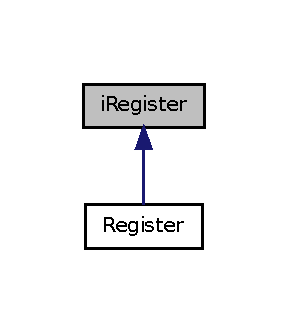
\includegraphics[width=136pt]{classiRegister__inherit__graph}
\end{center}
\end{figure}
\subsection*{Public Member Functions}
\begin{DoxyCompactItemize}
\item 
virtual \hyperlink{classWord}{Word} \hyperlink{classiRegister_ae7266f6f981b621f53f3c7cf77d4966a}{GetValue} () const =0
\begin{DoxyCompactList}\small\item\em Retrieves a copy of the word of data store in the register. \item\end{DoxyCompactList}\item 
virtual void \hyperlink{classiRegister_acb13aa880933f43088958723c9d6e564}{Add} (const \hyperlink{classiWord}{iWord} \&w)=0
\begin{DoxyCompactList}\small\item\em Adds a word of data to the calling object. \item\end{DoxyCompactList}\item 
virtual \hyperlink{classRegister}{Register} \hyperlink{classiRegister_abaaacfa8cb18bea90a78673bd572a1c8}{Add} (const \hyperlink{classiRegister}{iRegister} \&r) const =0
\begin{DoxyCompactList}\small\item\em Adds a word of data to the calling object. \item\end{DoxyCompactList}\item 
virtual \hyperlink{classRegister}{Register} \hyperlink{classiRegister_af8ab19234f44a0bade65cb35fd2cd036}{operator+} (const \hyperlink{classiRegister}{iRegister} \&r) const =0
\begin{DoxyCompactList}\small\item\em A standard add operator. \item\end{DoxyCompactList}\item 
virtual void \hyperlink{classiRegister_a98de346c2d0b15bee47d76bc5f70e94b}{Subtract} (const \hyperlink{classiWord}{iWord} \&w)=0
\begin{DoxyCompactList}\small\item\em Subtracts a word of data from the calling object. \item\end{DoxyCompactList}\item 
virtual \hyperlink{classRegister}{Register} \hyperlink{classiRegister_ad7eb424400d184f1829664dd4f87ce5c}{Subtract} (const \hyperlink{classiRegister}{iRegister} \&r) const =0
\begin{DoxyCompactList}\small\item\em Subtracts a word of data from the calling object. \item\end{DoxyCompactList}\item 
virtual \hyperlink{classRegister}{Register} \hyperlink{classiRegister_a01f837097cb87ec33fdc1cef606e1842}{operator-\/} (const \hyperlink{classiRegister}{iRegister} \&r) const =0
\begin{DoxyCompactList}\small\item\em A standard subtraction operator. \item\end{DoxyCompactList}\item 
virtual void \hyperlink{classiRegister_ae8114106e70653a705f04ba3892ed9e1}{And} (const \hyperlink{classiWord}{iWord} \&w)=0
\begin{DoxyCompactList}\small\item\em Performs a bit-\/wise and. \item\end{DoxyCompactList}\item 
virtual \hyperlink{classRegister}{Register} \hyperlink{classiRegister_aa9a15ebfeea1e5857a1098b73cc583ad}{And} (const \hyperlink{classiRegister}{iRegister} \&r) const =0
\begin{DoxyCompactList}\small\item\em Performs a bit-\/wise and. \item\end{DoxyCompactList}\item 
virtual void \hyperlink{classiRegister_aa0eac4fe58bde4a280a42fda1c087eee}{Or} (const \hyperlink{classiWord}{iWord} \&w)=0
\begin{DoxyCompactList}\small\item\em Performs a bit-\/wise \char`\"{}or\char`\"{}. \item\end{DoxyCompactList}\item 
virtual \hyperlink{classRegister}{Register} \hyperlink{classiRegister_af5f065e89ef31d2ed40a1e80d9231bfd}{Or} (const \hyperlink{classiRegister}{iRegister} \&r) const =0
\begin{DoxyCompactList}\small\item\em Performs a bit-\/wise or. \item\end{DoxyCompactList}\item 
virtual void \hyperlink{classiRegister_af4bbbe945b151dee3f1743c43a451cb3}{Not} ()=0
\begin{DoxyCompactList}\small\item\em Performs a bit-\/wise not. \item\end{DoxyCompactList}\item 
virtual \hyperlink{classRegister}{Register} \hyperlink{classiRegister_aca99e377de5cd1ef136a850d85143cf3}{Not} () const =0
\begin{DoxyCompactList}\small\item\em Performs a bit-\/wise not. \item\end{DoxyCompactList}\item 
virtual void \hyperlink{classiRegister_a8ffac24d1d7326e1a15f9b37cd426969}{Store} (const \hyperlink{classiWord}{iWord} \&w)=0
\begin{DoxyCompactList}\small\item\em Stores a word of data. \item\end{DoxyCompactList}\item 
virtual void \hyperlink{classiRegister_ac2b021b80a890f010fc68826e29fee47}{Store} (const \hyperlink{classiRegister}{iRegister} \&r)=0
\begin{DoxyCompactList}\small\item\em Stores a copy of another register. \item\end{DoxyCompactList}\item 
virtual \hyperlink{classRegister}{Register} \& \hyperlink{classiRegister_a16bf3f305a9588ddc85c109ac9a8b47b}{operator=} (const \hyperlink{classiWord}{iWord} \&w)=0
\begin{DoxyCompactList}\small\item\em A standard assignment operator. \item\end{DoxyCompactList}\item 
virtual \hyperlink{classRegister}{Register} \& \hyperlink{classiRegister_a3280dc5af6b828d875c57c3a3eac54d9}{operator=} (const \hyperlink{classRegister}{Register} r)=0
\begin{DoxyCompactList}\small\item\em A standard assignment operator. \item\end{DoxyCompactList}\item 
virtual \hyperlink{classRegister}{Register} \& \hyperlink{classiRegister_abca2bcea556d63fb4e3504df221cdc62}{operator++} ()=0
\begin{DoxyCompactList}\small\item\em A standard pre-\/increment operator. \item\end{DoxyCompactList}\item 
virtual \hyperlink{classRegister}{Register} \& \hyperlink{classiRegister_a36e6e1bfbc6a9fe203e8fb5b9f6396cb}{operator++} (int)=0
\begin{DoxyCompactList}\small\item\em A standard post-\/increment operator. \item\end{DoxyCompactList}\end{DoxyCompactItemize}


\subsection{Detailed Description}
Defines a \char`\"{}register\char`\"{} in the Wi-\/11 machine. The methods present in this inteface are meant to mimic the functionality of the Wi-\/11 machine, allowing for simplified execution of the instructions therein. This interace class will serve as a base from which the general purpose registers and program counter of the Wi-\/11 can be defined. 

\subsection{Member Function Documentation}
\hypertarget{classiRegister_ae7266f6f981b621f53f3c7cf77d4966a}{
\index{iRegister@{iRegister}!GetValue@{GetValue}}
\index{GetValue@{GetValue}!iRegister@{iRegister}}
\subsubsection[{GetValue}]{\setlength{\rightskip}{0pt plus 5cm}virtual {\bf Word} iRegister::GetValue (
\begin{DoxyParamCaption}
{}
\end{DoxyParamCaption}
) const\hspace{0.3cm}{\ttfamily  \mbox{[}pure virtual\mbox{]}}}}
\label{classiRegister_ae7266f6f981b621f53f3c7cf77d4966a}


Retrieves a copy of the word of data store in the register. 

\begin{DoxyPostcond}{Postcondition}
The value of the calling object is not changed. 
\end{DoxyPostcond}
\begin{DoxyReturn}{Returns}
A new \hyperlink{classWord}{Word} object holding the value that is stored in the register. 
\end{DoxyReturn}


Implemented in \hyperlink{classRegister_a379734c28ab8258ce528a96de24cfa1a}{Register}.

\hypertarget{classiRegister_acb13aa880933f43088958723c9d6e564}{
\index{iRegister@{iRegister}!Add@{Add}}
\index{Add@{Add}!iRegister@{iRegister}}
\subsubsection[{Add}]{\setlength{\rightskip}{0pt plus 5cm}virtual void iRegister::Add (
\begin{DoxyParamCaption}
\item[{const {\bf iWord} \&}]{ w}
\end{DoxyParamCaption}
)\hspace{0.3cm}{\ttfamily  \mbox{[}pure virtual\mbox{]}}}}
\label{classiRegister_acb13aa880933f43088958723c9d6e564}


Adds a word of data to the calling object. 


\begin{DoxyParams}[1]{Parameters}
\mbox{\tt in}  & {\em w} & The value to be added. \\
\hline
\end{DoxyParams}
\begin{DoxyPostcond}{Postcondition}
The calling object equals its previous value plus the value of \char`\"{}w\char`\"{}; \char`\"{}w\char`\"{}, however, will remain unchanged. 
\end{DoxyPostcond}


Implemented in \hyperlink{classRegister_a73d8564754d7ddb7e8349001010e688b}{Register}.

\hypertarget{classiRegister_abaaacfa8cb18bea90a78673bd572a1c8}{
\index{iRegister@{iRegister}!Add@{Add}}
\index{Add@{Add}!iRegister@{iRegister}}
\subsubsection[{Add}]{\setlength{\rightskip}{0pt plus 5cm}virtual {\bf Register} iRegister::Add (
\begin{DoxyParamCaption}
\item[{const {\bf iRegister} \&}]{ r}
\end{DoxyParamCaption}
) const\hspace{0.3cm}{\ttfamily  \mbox{[}pure virtual\mbox{]}}}}
\label{classiRegister_abaaacfa8cb18bea90a78673bd572a1c8}


Adds a word of data to the calling object. 


\begin{DoxyParams}[1]{Parameters}
\mbox{\tt in}  & {\em r} & The value to be added. \\
\hline
\end{DoxyParams}
\begin{DoxyPostcond}{Postcondition}
Both the calling object and \char`\"{}r\char`\"{} will not be changed. 
\end{DoxyPostcond}
\begin{DoxyReturn}{Returns}
A new \hyperlink{classRegister}{Register} object holding the value of the calling object plus the value in \char`\"{}r\char`\"{}. 
\end{DoxyReturn}


Implemented in \hyperlink{classRegister_a9d9c6801db55e8706eb242b1e0e0fa3f}{Register}.

\hypertarget{classiRegister_af8ab19234f44a0bade65cb35fd2cd036}{
\index{iRegister@{iRegister}!operator+@{operator+}}
\index{operator+@{operator+}!iRegister@{iRegister}}
\subsubsection[{operator+}]{\setlength{\rightskip}{0pt plus 5cm}virtual {\bf Register} iRegister::operator+ (
\begin{DoxyParamCaption}
\item[{const {\bf iRegister} \&}]{ r}
\end{DoxyParamCaption}
) const\hspace{0.3cm}{\ttfamily  \mbox{[}pure virtual\mbox{]}}}}
\label{classiRegister_af8ab19234f44a0bade65cb35fd2cd036}


A standard add operator. 

\begin{DoxyNote}{Note}
\char`\"{}result = p + r\char`\"{} is equivalent to \char`\"{}result = p.Add(r)\char`\"{}. 
\end{DoxyNote}


Implemented in \hyperlink{classRegister_a55de0c3b5f8fe14df7c24bce777204e0}{Register}.

\hypertarget{classiRegister_a98de346c2d0b15bee47d76bc5f70e94b}{
\index{iRegister@{iRegister}!Subtract@{Subtract}}
\index{Subtract@{Subtract}!iRegister@{iRegister}}
\subsubsection[{Subtract}]{\setlength{\rightskip}{0pt plus 5cm}virtual void iRegister::Subtract (
\begin{DoxyParamCaption}
\item[{const {\bf iWord} \&}]{ w}
\end{DoxyParamCaption}
)\hspace{0.3cm}{\ttfamily  \mbox{[}pure virtual\mbox{]}}}}
\label{classiRegister_a98de346c2d0b15bee47d76bc5f70e94b}


Subtracts a word of data from the calling object. 


\begin{DoxyParams}[1]{Parameters}
\mbox{\tt in}  & {\em w} & The value to be subtracted. \\
\hline
\end{DoxyParams}
\begin{DoxyPostcond}{Postcondition}
The calling object equals its previous value minus the value of \char`\"{}w\char`\"{}; \char`\"{}w\char`\"{}, however, will remain unchanged. 
\end{DoxyPostcond}


Implemented in \hyperlink{classRegister_a726a720b6bcca282945f1c0a65ca0dd4}{Register}.

\hypertarget{classiRegister_ad7eb424400d184f1829664dd4f87ce5c}{
\index{iRegister@{iRegister}!Subtract@{Subtract}}
\index{Subtract@{Subtract}!iRegister@{iRegister}}
\subsubsection[{Subtract}]{\setlength{\rightskip}{0pt plus 5cm}virtual {\bf Register} iRegister::Subtract (
\begin{DoxyParamCaption}
\item[{const {\bf iRegister} \&}]{ r}
\end{DoxyParamCaption}
) const\hspace{0.3cm}{\ttfamily  \mbox{[}pure virtual\mbox{]}}}}
\label{classiRegister_ad7eb424400d184f1829664dd4f87ce5c}


Subtracts a word of data from the calling object. 


\begin{DoxyParams}[1]{Parameters}
\mbox{\tt in}  & {\em r} & The value to be subtracted. \\
\hline
\end{DoxyParams}
\begin{DoxyPostcond}{Postcondition}
Both the calling object and \char`\"{}r\char`\"{} will not be changed. 
\end{DoxyPostcond}
\begin{DoxyReturn}{Returns}
A new \hyperlink{classRegister}{Register} object holding the value of the calling object minus the value in \char`\"{}r\char`\"{}. 
\end{DoxyReturn}


Implemented in \hyperlink{classRegister_a05132a4a62f5c6883fdf78731970ab6a}{Register}.

\hypertarget{classiRegister_a01f837097cb87ec33fdc1cef606e1842}{
\index{iRegister@{iRegister}!operator-\/@{operator-\/}}
\index{operator-\/@{operator-\/}!iRegister@{iRegister}}
\subsubsection[{operator-\/}]{\setlength{\rightskip}{0pt plus 5cm}virtual {\bf Register} iRegister::operator-\/ (
\begin{DoxyParamCaption}
\item[{const {\bf iRegister} \&}]{ r}
\end{DoxyParamCaption}
) const\hspace{0.3cm}{\ttfamily  \mbox{[}pure virtual\mbox{]}}}}
\label{classiRegister_a01f837097cb87ec33fdc1cef606e1842}


A standard subtraction operator. 

\begin{DoxyNote}{Note}
\char`\"{}result = p -\/ r\char`\"{} is equivalent to \char`\"{}result = r.Subtract(w)\char`\"{}. 
\end{DoxyNote}


Implemented in \hyperlink{classRegister_a43c957e4b6a3103f0634258891c82b46}{Register}.

\hypertarget{classiRegister_ae8114106e70653a705f04ba3892ed9e1}{
\index{iRegister@{iRegister}!And@{And}}
\index{And@{And}!iRegister@{iRegister}}
\subsubsection[{And}]{\setlength{\rightskip}{0pt plus 5cm}virtual void iRegister::And (
\begin{DoxyParamCaption}
\item[{const {\bf iWord} \&}]{ w}
\end{DoxyParamCaption}
)\hspace{0.3cm}{\ttfamily  \mbox{[}pure virtual\mbox{]}}}}
\label{classiRegister_ae8114106e70653a705f04ba3892ed9e1}


Performs a bit-\/wise and. 


\begin{DoxyParams}[1]{Parameters}
\mbox{\tt in}  & {\em w} & The value to be \char`\"{}and\char`\"{}ed. \\
\hline
\end{DoxyParams}
\begin{DoxyPostcond}{Postcondition}
The calling object equals its previous value bit-\/wise and'ed with w. 
\end{DoxyPostcond}


Implemented in \hyperlink{classRegister_a312263efb06ef459409879f5119b3b81}{Register}.

\hypertarget{classiRegister_aa9a15ebfeea1e5857a1098b73cc583ad}{
\index{iRegister@{iRegister}!And@{And}}
\index{And@{And}!iRegister@{iRegister}}
\subsubsection[{And}]{\setlength{\rightskip}{0pt plus 5cm}virtual {\bf Register} iRegister::And (
\begin{DoxyParamCaption}
\item[{const {\bf iRegister} \&}]{ r}
\end{DoxyParamCaption}
) const\hspace{0.3cm}{\ttfamily  \mbox{[}pure virtual\mbox{]}}}}
\label{classiRegister_aa9a15ebfeea1e5857a1098b73cc583ad}


Performs a bit-\/wise and. 


\begin{DoxyParams}[1]{Parameters}
\mbox{\tt in}  & {\em r} & The value to be \char`\"{}and\char`\"{}ed. \\
\hline
\end{DoxyParams}
\begin{DoxyPostcond}{Postcondition}
Both the calling object and r are not changed. 
\end{DoxyPostcond}
\begin{DoxyReturn}{Returns}
A new \hyperlink{classRegister}{Register} object holding the value of the calling object bit-\/wise and'ed with r. 
\end{DoxyReturn}


Implemented in \hyperlink{classRegister_af3502239502c214b8c9362a6fd9f8ff8}{Register}.

\hypertarget{classiRegister_aa0eac4fe58bde4a280a42fda1c087eee}{
\index{iRegister@{iRegister}!Or@{Or}}
\index{Or@{Or}!iRegister@{iRegister}}
\subsubsection[{Or}]{\setlength{\rightskip}{0pt plus 5cm}virtual void iRegister::Or (
\begin{DoxyParamCaption}
\item[{const {\bf iWord} \&}]{ w}
\end{DoxyParamCaption}
)\hspace{0.3cm}{\ttfamily  \mbox{[}pure virtual\mbox{]}}}}
\label{classiRegister_aa0eac4fe58bde4a280a42fda1c087eee}


Performs a bit-\/wise \char`\"{}or\char`\"{}. 


\begin{DoxyParams}[1]{Parameters}
\mbox{\tt in}  & {\em w} & The value to be \char`\"{}or\char`\"{}ed. \\
\hline
\end{DoxyParams}
\begin{DoxyPostcond}{Postcondition}
The calling object equals its previous value bit-\/wise or'ed with w. 
\end{DoxyPostcond}


Implemented in \hyperlink{classRegister_ab2f8407fab157d8deea936fa74424115}{Register}.

\hypertarget{classiRegister_af5f065e89ef31d2ed40a1e80d9231bfd}{
\index{iRegister@{iRegister}!Or@{Or}}
\index{Or@{Or}!iRegister@{iRegister}}
\subsubsection[{Or}]{\setlength{\rightskip}{0pt plus 5cm}virtual {\bf Register} iRegister::Or (
\begin{DoxyParamCaption}
\item[{const {\bf iRegister} \&}]{ r}
\end{DoxyParamCaption}
) const\hspace{0.3cm}{\ttfamily  \mbox{[}pure virtual\mbox{]}}}}
\label{classiRegister_af5f065e89ef31d2ed40a1e80d9231bfd}


Performs a bit-\/wise or. 


\begin{DoxyParams}[1]{Parameters}
\mbox{\tt in}  & {\em r} & The value to be \char`\"{}or\char`\"{}ed. \\
\hline
\end{DoxyParams}
\begin{DoxyPostcond}{Postcondition}
Both the calling object and r are not changed. 
\end{DoxyPostcond}
\begin{DoxyReturn}{Returns}
A new \hyperlink{classRegister}{Register} object holding the value of the calling object bit-\/wise or'ed with r. 
\end{DoxyReturn}


Implemented in \hyperlink{classRegister_a9400801cc625144c4606cd7f5cbbaa21}{Register}.

\hypertarget{classiRegister_af4bbbe945b151dee3f1743c43a451cb3}{
\index{iRegister@{iRegister}!Not@{Not}}
\index{Not@{Not}!iRegister@{iRegister}}
\subsubsection[{Not}]{\setlength{\rightskip}{0pt plus 5cm}virtual void iRegister::Not (
\begin{DoxyParamCaption}
{}
\end{DoxyParamCaption}
)\hspace{0.3cm}{\ttfamily  \mbox{[}pure virtual\mbox{]}}}}
\label{classiRegister_af4bbbe945b151dee3f1743c43a451cb3}


Performs a bit-\/wise not. 

\begin{DoxyPostcond}{Postcondition}
The calling object's bits are all flipped (e.g. 1001 -\/$>$ 0110). 
\end{DoxyPostcond}


Implemented in \hyperlink{classRegister_abbf5f6793328db8b28845cac84c0e82d}{Register}.

\hypertarget{classiRegister_aca99e377de5cd1ef136a850d85143cf3}{
\index{iRegister@{iRegister}!Not@{Not}}
\index{Not@{Not}!iRegister@{iRegister}}
\subsubsection[{Not}]{\setlength{\rightskip}{0pt plus 5cm}virtual {\bf Register} iRegister::Not (
\begin{DoxyParamCaption}
{}
\end{DoxyParamCaption}
) const\hspace{0.3cm}{\ttfamily  \mbox{[}pure virtual\mbox{]}}}}
\label{classiRegister_aca99e377de5cd1ef136a850d85143cf3}


Performs a bit-\/wise not. 

\begin{DoxyPostcond}{Postcondition}
The calling object is not changed. 
\end{DoxyPostcond}
\begin{DoxyReturn}{Returns}
A new \hyperlink{classRegister}{Register} object holding the bit-\/wise not of the calling object. 
\end{DoxyReturn}


Implemented in \hyperlink{classRegister_a387bb50d01b47071c366708ea10ebdf0}{Register}.

\hypertarget{classiRegister_a8ffac24d1d7326e1a15f9b37cd426969}{
\index{iRegister@{iRegister}!Store@{Store}}
\index{Store@{Store}!iRegister@{iRegister}}
\subsubsection[{Store}]{\setlength{\rightskip}{0pt plus 5cm}virtual void iRegister::Store (
\begin{DoxyParamCaption}
\item[{const {\bf iWord} \&}]{ w}
\end{DoxyParamCaption}
)\hspace{0.3cm}{\ttfamily  \mbox{[}pure virtual\mbox{]}}}}
\label{classiRegister_a8ffac24d1d7326e1a15f9b37cd426969}


Stores a word of data. 


\begin{DoxyParams}[1]{Parameters}
\mbox{\tt in}  & {\em w} & The value to be store. \\
\hline
\end{DoxyParams}
\begin{DoxyPostcond}{Postcondition}
The calling object's value is now \char`\"{}w\char`\"{}. 
\end{DoxyPostcond}


Implemented in \hyperlink{classRegister_affcc16cc88cdc896803b1ab6af5d38e0}{Register}.

\hypertarget{classiRegister_ac2b021b80a890f010fc68826e29fee47}{
\index{iRegister@{iRegister}!Store@{Store}}
\index{Store@{Store}!iRegister@{iRegister}}
\subsubsection[{Store}]{\setlength{\rightskip}{0pt plus 5cm}virtual void iRegister::Store (
\begin{DoxyParamCaption}
\item[{const {\bf iRegister} \&}]{ r}
\end{DoxyParamCaption}
)\hspace{0.3cm}{\ttfamily  \mbox{[}pure virtual\mbox{]}}}}
\label{classiRegister_ac2b021b80a890f010fc68826e29fee47}


Stores a copy of another register. 


\begin{DoxyParams}[1]{Parameters}
\mbox{\tt in}  & {\em r} & The register to be copied. \\
\hline
\end{DoxyParams}
\begin{DoxyPostcond}{Postcondition}
The calling object's value is now \char`\"{}r\char`\"{}. 
\end{DoxyPostcond}


Implemented in \hyperlink{classRegister_a2ac7bd6f2e0eb38800c0a8c8d045e18e}{Register}.

\hypertarget{classiRegister_a16bf3f305a9588ddc85c109ac9a8b47b}{
\index{iRegister@{iRegister}!operator=@{operator=}}
\index{operator=@{operator=}!iRegister@{iRegister}}
\subsubsection[{operator=}]{\setlength{\rightskip}{0pt plus 5cm}virtual {\bf Register}\& iRegister::operator= (
\begin{DoxyParamCaption}
\item[{const {\bf iWord} \&}]{ w}
\end{DoxyParamCaption}
)\hspace{0.3cm}{\ttfamily  \mbox{[}pure virtual\mbox{]}}}}
\label{classiRegister_a16bf3f305a9588ddc85c109ac9a8b47b}


A standard assignment operator. 

\begin{DoxyNote}{Note}
\char`\"{}r = w\char`\"{} is equivalent to \char`\"{}r.Store(w)\char`\"{} 
\end{DoxyNote}


Implemented in \hyperlink{classRegister_afc5f775405700146638e392d81ad7d0b}{Register}.

\hypertarget{classiRegister_a3280dc5af6b828d875c57c3a3eac54d9}{
\index{iRegister@{iRegister}!operator=@{operator=}}
\index{operator=@{operator=}!iRegister@{iRegister}}
\subsubsection[{operator=}]{\setlength{\rightskip}{0pt plus 5cm}virtual {\bf Register}\& iRegister::operator= (
\begin{DoxyParamCaption}
\item[{const {\bf Register}}]{ r}
\end{DoxyParamCaption}
)\hspace{0.3cm}{\ttfamily  \mbox{[}pure virtual\mbox{]}}}}
\label{classiRegister_a3280dc5af6b828d875c57c3a3eac54d9}


A standard assignment operator. 

\begin{DoxyNote}{Note}
\char`\"{}r1 = r2\char`\"{} is equivalent to \char`\"{}r1.Store(r2)\char`\"{} 
\end{DoxyNote}


Implemented in \hyperlink{classRegister_a00f7aaf798102e5c7a6fb311551b492f}{Register}.

\hypertarget{classiRegister_abca2bcea556d63fb4e3504df221cdc62}{
\index{iRegister@{iRegister}!operator++@{operator++}}
\index{operator++@{operator++}!iRegister@{iRegister}}
\subsubsection[{operator++}]{\setlength{\rightskip}{0pt plus 5cm}virtual {\bf Register}\& iRegister::operator++ (
\begin{DoxyParamCaption}
{}
\end{DoxyParamCaption}
)\hspace{0.3cm}{\ttfamily  \mbox{[}pure virtual\mbox{]}}}}
\label{classiRegister_abca2bcea556d63fb4e3504df221cdc62}


A standard pre-\/increment operator. 

\begin{DoxyReturn}{Returns}
A reference to itself.
\end{DoxyReturn}
The object increments its value BEFORE the execution of the current line. 

Implemented in \hyperlink{classRegister_ac4e78cff131bc5c69695a9db5ca35255}{Register}.

\hypertarget{classiRegister_a36e6e1bfbc6a9fe203e8fb5b9f6396cb}{
\index{iRegister@{iRegister}!operator++@{operator++}}
\index{operator++@{operator++}!iRegister@{iRegister}}
\subsubsection[{operator++}]{\setlength{\rightskip}{0pt plus 5cm}virtual {\bf Register}\& iRegister::operator++ (
\begin{DoxyParamCaption}
\item[{int}]{}
\end{DoxyParamCaption}
)\hspace{0.3cm}{\ttfamily  \mbox{[}pure virtual\mbox{]}}}}
\label{classiRegister_a36e6e1bfbc6a9fe203e8fb5b9f6396cb}


A standard post-\/increment operator. 

\begin{DoxyReturn}{Returns}
A reference to itself.
\end{DoxyReturn}
The object increments its value AFTER the execution of the current line. 

Implemented in \hyperlink{classRegister_ae3414befdccf70a18df0f67dc19d86b7}{Register}.


\hypertarget{classiSimulator}{
\section{iSimulator Class Reference}
\label{classiSimulator}\index{iSimulator@{iSimulator}}
}
\subsection*{Public Member Functions}
\begin{DoxyCompactItemize}
\item 
\hypertarget{classiSimulator_a26f260b37ec3da3d35624ef6d69c8e43}{
virtual bool {\bfseries Initialize} (const char $\ast$)=0}
\label{classiSimulator_a26f260b37ec3da3d35624ef6d69c8e43}

\item 
\hypertarget{classiSimulator_a7a8fbaee266ec14b2c15888ebb325bd2}{
virtual bool {\bfseries Add} (const REGISTER\_\-ID DR, const REGISTER\_\-ID SR1, const REGISTER\_\-ID SR2)=0}
\label{classiSimulator_a7a8fbaee266ec14b2c15888ebb325bd2}

\item 
\hypertarget{classiSimulator_a632a5d1627f9947f04972caa2d532751}{
virtual bool {\bfseries Add} (const REGISTER\_\-ID DR, const REGISTER\_\-ID SR1, const \hyperlink{classiWord}{iWord} \&immediate)=0}
\label{classiSimulator_a632a5d1627f9947f04972caa2d532751}

\item 
\hypertarget{classiSimulator_acc1c5c681d3ee7b810ef0e5255aa80e5}{
virtual bool {\bfseries And} (const REGISTER\_\-ID DR, const REGISTER\_\-ID SR1, const REGISTER\_\-ID SR2)=0}
\label{classiSimulator_acc1c5c681d3ee7b810ef0e5255aa80e5}

\item 
\hypertarget{classiSimulator_afe859dbd05cff55c12fd3f693a78e9a3}{
virtual bool {\bfseries And} (const REGISTER\_\-ID DR, const REGISTER\_\-ID SR1, const \hyperlink{classiWord}{iWord} \&immediate)=0}
\label{classiSimulator_afe859dbd05cff55c12fd3f693a78e9a3}

\item 
\hypertarget{classiSimulator_a4377a067039a3501ea4cd02602ef10d0}{
virtual bool {\bfseries Branch} (const \hyperlink{classiWord}{iWord} \&address)=0}
\label{classiSimulator_a4377a067039a3501ea4cd02602ef10d0}

\item 
\hypertarget{classiSimulator_a8535c27de33581067925bcea28b2585d}{
virtual bool {\bfseries Debug} ()=0}
\label{classiSimulator_a8535c27de33581067925bcea28b2585d}

\item 
\hypertarget{classiSimulator_ab30229a9093f96ae8f49e4a82b2f0a96}{
virtual bool {\bfseries JSR} (const \hyperlink{classiWord}{iWord} \&)=0}
\label{classiSimulator_ab30229a9093f96ae8f49e4a82b2f0a96}

\item 
\hypertarget{classiSimulator_a9f4b0281a3f3d7f0a17f6163926af0fe}{
virtual bool {\bfseries JSRR} (const \hyperlink{classiWord}{iWord} \&baseR, const \hyperlink{classiWord}{iWord} \&address)=0}
\label{classiSimulator_a9f4b0281a3f3d7f0a17f6163926af0fe}

\item 
\hypertarget{classiSimulator_aebed4efd384ed7a2058a331abb443de3}{
virtual bool {\bfseries Load} (const REGISTER\_\-ID DR, const \hyperlink{classiWord}{iWord} \&address)=0}
\label{classiSimulator_aebed4efd384ed7a2058a331abb443de3}

\item 
\hypertarget{classiSimulator_ac9d482f3e08540a0e753ac07ad184f0c}{
virtual bool {\bfseries LDI} (const REGISTER\_\-ID DR, const \hyperlink{classiWord}{iWord} \&address)=0}
\label{classiSimulator_ac9d482f3e08540a0e753ac07ad184f0c}

\item 
\hypertarget{classiSimulator_a3008e18326b41cdd8226da07b9409b62}{
virtual bool {\bfseries LDR} (const REGISTER\_\-ID DR, const \hyperlink{classiWord}{iWord} \&baseR, const \hyperlink{classiWord}{iWord} \&address)=0}
\label{classiSimulator_a3008e18326b41cdd8226da07b9409b62}

\item 
\hypertarget{classiSimulator_a8d418321f4eef73d5cf3b17ac64c0ba8}{
virtual bool {\bfseries Not} (const REGISTER\_\-ID DR, const REGISTER\_\-ID SR)=0}
\label{classiSimulator_a8d418321f4eef73d5cf3b17ac64c0ba8}

\item 
\hypertarget{classiSimulator_a272e6a7baebbb777bdeb60d67e4fcb17}{
virtual bool {\bfseries Ret} ()=0}
\label{classiSimulator_a272e6a7baebbb777bdeb60d67e4fcb17}

\item 
\hypertarget{classiSimulator_a8b43cb8d1da6eefc49d629bf744837d3}{
virtual bool {\bfseries Store} (const REGISTER\_\-ID DR, const \hyperlink{classiWord}{iWord} \&address)=0}
\label{classiSimulator_a8b43cb8d1da6eefc49d629bf744837d3}

\item 
\hypertarget{classiSimulator_aa434d5add2b2b98ad301a1c842fb158f}{
virtual bool {\bfseries STI} (const REGISTER\_\-ID DR, const \hyperlink{classiWord}{iWord} \&address)=0}
\label{classiSimulator_aa434d5add2b2b98ad301a1c842fb158f}

\item 
\hypertarget{classiSimulator_aec50c2cc4b7fc2429bfa62ddc79d41df}{
virtual bool {\bfseries STR} (const REGISTER\_\-ID DR, const \hyperlink{classiWord}{iWord} \&baseR, const \hyperlink{classiWord}{iWord} \&address)=0}
\label{classiSimulator_aec50c2cc4b7fc2429bfa62ddc79d41df}

\item 
\hypertarget{classiSimulator_a9ddfcfe7f0c1d563193b096e1058e388}{
virtual bool {\bfseries Trap} (const \hyperlink{classiWord}{iWord} \&address)=0}
\label{classiSimulator_a9ddfcfe7f0c1d563193b096e1058e388}

\end{DoxyCompactItemize}


The documentation for this class was generated from the following file:\begin{DoxyCompactItemize}
\item 
iSimulator.h\end{DoxyCompactItemize}

\hypertarget{classiWord}{
\section{iWord Class Reference}
\label{classiWord}\index{iWord@{iWord}}
}


The \hyperlink{classiWord}{iWord} interface class defines the a \char`\"{}word\char`\"{} of data on the Wi-\/11 Machine.  




Inheritance diagram for iWord:\nopagebreak
\begin{figure}[H]
\begin{center}
\leavevmode
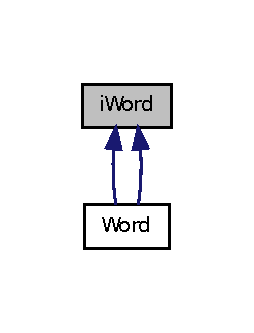
\includegraphics[width=122pt]{classiWord__inherit__graph}
\end{center}
\end{figure}
\subsection*{Public Member Functions}
\begin{DoxyCompactItemize}
\item 
virtual int \hyperlink{classiWord_a3349d0a243d3432bb35b76af8420b1d9}{toInt} () const =0
\begin{DoxyCompactList}\small\item\em \char`\"{}To non-\/negative Integer\char`\"{} \item\end{DoxyCompactList}\item 
virtual int \hyperlink{classiWord_a1377d01257b792c748b013be60b089e6}{toInt2Complement} () const =0
\begin{DoxyCompactList}\small\item\em \char`\"{}To Integer as 2's Complement\char`\"{} \item\end{DoxyCompactList}\item 
virtual std::string \hyperlink{classiWord_a0114861c4b660286834ad637f11dc4f4}{toStr} () const =0
\begin{DoxyCompactList}\small\item\em \char`\"{}To String\char`\"{} \item\end{DoxyCompactList}\item 
virtual std::string \hyperlink{classiWord_a7fc28d0251f8acb4dc3f388fc25c57d1}{toHex} () const =0
\begin{DoxyCompactList}\small\item\em \char`\"{}To Hexadecimal\char`\"{} \item\end{DoxyCompactList}\item 
virtual bool \hyperlink{classiWord_a6421bf139c6eb4044446997606cb65e7}{fromInt} (int)=0
\begin{DoxyCompactList}\small\item\em \char`\"{}From Integer\char`\"{} \item\end{DoxyCompactList}\item 
virtual bool \hyperlink{classiWord_ad8df9e06ccb87d1e65766120713ef545}{fromStr} (const std::string \&)=0
\begin{DoxyCompactList}\small\item\em \char`\"{}From String\char`\"{} \item\end{DoxyCompactList}\item 
virtual bool \hyperlink{classiWord_a0c08832b3e9b41073fc6666407ef8c53}{fromHex} (const std::string \&)=0
\begin{DoxyCompactList}\small\item\em \char`\"{}From Hexadecimal\char`\"{} \item\end{DoxyCompactList}\item 
virtual \hyperlink{classWord}{Word} \hyperlink{classiWord_a999c52ac2e7abf756eeb16fe5b31aad7}{Add} (const \hyperlink{classiWord}{iWord} \&) const =0
\begin{DoxyCompactList}\small\item\em Adds two words. \item\end{DoxyCompactList}\item 
virtual \hyperlink{classWord}{Word} \hyperlink{classiWord_a8dfb66b7cd91fe0a4169f071c1f9bc53}{operator+} (const \hyperlink{classiWord}{iWord} \&) const =0
\begin{DoxyCompactList}\small\item\em A standard addition operator. \item\end{DoxyCompactList}\item 
virtual \hyperlink{classWord}{Word} \hyperlink{classiWord_af69a5e10e094e3fc30fae0b651d95ea6}{Subtract} (const \hyperlink{classiWord}{iWord} \&) const =0
\begin{DoxyCompactList}\small\item\em Subtracts two words. \item\end{DoxyCompactList}\item 
virtual \hyperlink{classWord}{Word} \hyperlink{classiWord_a432fb05081debadb601d86cca05152c8}{operator-\/} (const \hyperlink{classiWord}{iWord} \&) const =0
\begin{DoxyCompactList}\small\item\em A standard subtraction operator. \item\end{DoxyCompactList}\item 
virtual \hyperlink{classWord}{Word} \hyperlink{classiWord_ae9f6bbc855712a208835d12cb3e40577}{And} (const \hyperlink{classiWord}{iWord} \&) const =0
\begin{DoxyCompactList}\small\item\em \char`\"{}And\char`\"{}s the bits of two words. \item\end{DoxyCompactList}\item 
\hypertarget{classiWord_a24a8821a44701deda1dd70972447172f}{
virtual \hyperlink{classWord}{Word} {\bfseries Or} (const \hyperlink{classiWord}{iWord} \&) const =0}
\label{classiWord_a24a8821a44701deda1dd70972447172f}

\item 
\hypertarget{classiWord_a6a7602a8220d84b5201a789b597fbbde}{
virtual \hyperlink{classWord}{Word} {\bfseries Not} () const =0}
\label{classiWord_a6a7602a8220d84b5201a789b597fbbde}

\item 
virtual void \hyperlink{classiWord_ab9f5df8ced4937c18f16784a98ecf95f}{copy} (const \hyperlink{classiWord}{iWord} \&)=0
\begin{DoxyCompactList}\small\item\em Copies a word. \item\end{DoxyCompactList}\item 
virtual \hyperlink{classWord}{Word} \& \hyperlink{classiWord_a45c9c82054bd2150b77d5f157734cb72}{operator=} (const \hyperlink{classWord}{Word})=0
\begin{DoxyCompactList}\small\item\em A standard assignment operator. \item\end{DoxyCompactList}\item 
virtual \hyperlink{classiWord}{iWord} \& \hyperlink{classiWord_af20040c25b79d2aeae41f1714fbb2cbc}{operator++} ()=0
\item 
virtual \hyperlink{classiWord}{iWord} \& \hyperlink{classiWord_a6777f6f41915179c4255d3647a9eb4b5}{operator++} (int)=0
\begin{DoxyCompactList}\small\item\em A standard post-\/increment operator. \item\end{DoxyCompactList}\item 
virtual bool \hyperlink{classiWord_a2bd140904379329b74c3e1af83eb3a85}{operator\mbox{[}$\,$\mbox{]}} (int) const =0
\begin{DoxyCompactList}\small\item\em An accessor to the \char`\"{}i\char`\"{}th bit of the value. \item\end{DoxyCompactList}\end{DoxyCompactItemize}


\subsection{Detailed Description}
The \hyperlink{classiWord}{iWord} interface class defines the a \char`\"{}word\char`\"{} of data on the Wi-\/11 Machine. The methods present in this inteface are meant to mimic the functionality of the Wi-\/11 machine, allowing for simplified execution of the instructions therein. As the size of a \char`\"{}word\char`\"{} depends on the architecture, classes implementing this interface should define the word length to be 16 bits in length. 

\subsection{Member Function Documentation}
\hypertarget{classiWord_a3349d0a243d3432bb35b76af8420b1d9}{
\index{iWord@{iWord}!toInt@{toInt}}
\index{toInt@{toInt}!iWord@{iWord}}
\subsubsection[{toInt}]{\setlength{\rightskip}{0pt plus 5cm}virtual int iWord::toInt (
\begin{DoxyParamCaption}
{}
\end{DoxyParamCaption}
) const\hspace{0.3cm}{\ttfamily  \mbox{[}pure virtual\mbox{]}}}}
\label{classiWord_a3349d0a243d3432bb35b76af8420b1d9}


\char`\"{}To non-\/negative Integer\char`\"{} 

\begin{DoxyPostcond}{Postcondition}
The value of the word is not changed. 
\end{DoxyPostcond}
\begin{DoxyReturn}{Returns}
The bits of the word interpreted as a positive integer value. 
\end{DoxyReturn}


Implemented in \hyperlink{classWord_a19303d963626549830a8da33d863bd6d}{Word}.

\hypertarget{classiWord_a1377d01257b792c748b013be60b089e6}{
\index{iWord@{iWord}!toInt2Complement@{toInt2Complement}}
\index{toInt2Complement@{toInt2Complement}!iWord@{iWord}}
\subsubsection[{toInt2Complement}]{\setlength{\rightskip}{0pt plus 5cm}virtual int iWord::toInt2Complement (
\begin{DoxyParamCaption}
{}
\end{DoxyParamCaption}
) const\hspace{0.3cm}{\ttfamily  \mbox{[}pure virtual\mbox{]}}}}
\label{classiWord_a1377d01257b792c748b013be60b089e6}


\char`\"{}To Integer as 2's Complement\char`\"{} 

\begin{DoxyPostcond}{Postcondition}
The value of the word is not changed. 
\end{DoxyPostcond}
\begin{DoxyReturn}{Returns}
The bits of the word interpreted as a signed (2's complement) integer value. 
\end{DoxyReturn}


Implemented in \hyperlink{classWord_a3d771d68afd4a70d279af8bd9cd6bef9}{Word}.

\hypertarget{classiWord_a0114861c4b660286834ad637f11dc4f4}{
\index{iWord@{iWord}!toStr@{toStr}}
\index{toStr@{toStr}!iWord@{iWord}}
\subsubsection[{toStr}]{\setlength{\rightskip}{0pt plus 5cm}virtual std::string iWord::toStr (
\begin{DoxyParamCaption}
{}
\end{DoxyParamCaption}
) const\hspace{0.3cm}{\ttfamily  \mbox{[}pure virtual\mbox{]}}}}
\label{classiWord_a0114861c4b660286834ad637f11dc4f4}


\char`\"{}To String\char`\"{} 

\begin{DoxyPostcond}{Postcondition}
The value of the word is not changed. 
\end{DoxyPostcond}
\begin{DoxyReturn}{Returns}
16 characters: each either a 1 or 0
\end{DoxyReturn}
\begin{DoxyParagraph}{Examples:}
If the object holds a (2's comp.) value 4: \char`\"{}0000000000000100\char`\"{}\par
 If the object holds a (2's comp.) value -\/1: \char`\"{}1111111111111111\char`\"{} 
\end{DoxyParagraph}


Implemented in \hyperlink{classWord_ac2ca49ef4da2fb57172fe057849e53fa}{Word}.

\hypertarget{classiWord_a7fc28d0251f8acb4dc3f388fc25c57d1}{
\index{iWord@{iWord}!toHex@{toHex}}
\index{toHex@{toHex}!iWord@{iWord}}
\subsubsection[{toHex}]{\setlength{\rightskip}{0pt plus 5cm}virtual std::string iWord::toHex (
\begin{DoxyParamCaption}
{}
\end{DoxyParamCaption}
) const\hspace{0.3cm}{\ttfamily  \mbox{[}pure virtual\mbox{]}}}}
\label{classiWord_a7fc28d0251f8acb4dc3f388fc25c57d1}


\char`\"{}To Hexadecimal\char`\"{} 

\begin{DoxyPostcond}{Postcondition}
The value of the word is not changed. 
\end{DoxyPostcond}
\begin{DoxyReturn}{Returns}
\char`\"{}0x\char`\"{} + $<$4 characters in the range \mbox{[}0-\/9\mbox{]},\mbox{[}A-\/F\mbox{]}$>$
\end{DoxyReturn}
\begin{DoxyParagraph}{Examples:}
If the object holds (2's comp.) value 8: \char`\"{}0x0008\char`\"{}\par
 If the object holds (2's comp.) value -\/2: \char`\"{}0xFFFE\char`\"{} 
\end{DoxyParagraph}


Implemented in \hyperlink{classWord_ab797467868642bb096bc4c9b1ed0a2f0}{Word}.

\hypertarget{classiWord_a6421bf139c6eb4044446997606cb65e7}{
\index{iWord@{iWord}!fromInt@{fromInt}}
\index{fromInt@{fromInt}!iWord@{iWord}}
\subsubsection[{fromInt}]{\setlength{\rightskip}{0pt plus 5cm}virtual bool iWord::fromInt (
\begin{DoxyParamCaption}
\item[{int}]{}
\end{DoxyParamCaption}
)\hspace{0.3cm}{\ttfamily  \mbox{[}pure virtual\mbox{]}}}}
\label{classiWord_a6421bf139c6eb4044446997606cb65e7}


\char`\"{}From Integer\char`\"{} 


\begin{DoxyParams}[1]{Parameters}
\mbox{\tt in}  & {\em value} & The value to be stored into the word. \\
\hline
\end{DoxyParams}
\begin{DoxyPostcond}{Postcondition}
\char`\"{}value\char`\"{} is not changed. 
\end{DoxyPostcond}
\begin{DoxyReturn}{Returns}
True if and only if \char`\"{}value\char`\"{} can be represented in 16 bits
\end{DoxyReturn}
When this function returns \char`\"{}False\char`\"{}, the value of the word is unchanged.\par
 Otherwise, the word now holds the value \char`\"{}value\char`\"{}. 

Implemented in \hyperlink{classWord_ad6499f93b487d6d550a3fd4adcee9c8d}{Word}.

\hypertarget{classiWord_ad8df9e06ccb87d1e65766120713ef545}{
\index{iWord@{iWord}!fromStr@{fromStr}}
\index{fromStr@{fromStr}!iWord@{iWord}}
\subsubsection[{fromStr}]{\setlength{\rightskip}{0pt plus 5cm}virtual bool iWord::fromStr (
\begin{DoxyParamCaption}
\item[{const std::string \&}]{}
\end{DoxyParamCaption}
)\hspace{0.3cm}{\ttfamily  \mbox{[}pure virtual\mbox{]}}}}
\label{classiWord_ad8df9e06ccb87d1e65766120713ef545}


\char`\"{}From String\char`\"{} 


\begin{DoxyParams}[1]{Parameters}
\mbox{\tt in}  & {\em str} & A string of characters meant to represent a \char`\"{}word\char`\"{} to be stored. \\
\hline
\end{DoxyParams}
\begin{DoxyPostcond}{Postcondition}
\char`\"{}str\char`\"{} is not changed. 
\end{DoxyPostcond}
\begin{DoxyReturn}{Returns}
True if and only if \char`\"{}str\char`\"{} is well-\/formed (as defined in \hyperlink{classiWord_a0114861c4b660286834ad637f11dc4f4}{toStr()}).
\end{DoxyReturn}
When this function returns \char`\"{}False\char`\"{}, the value of the word is unchanged.\par
 Otherwise, the word now holds the value \char`\"{}str\char`\"{}. 

Implemented in \hyperlink{classWord_a614b52f3312d82ac5681403651040714}{Word}.

\hypertarget{classiWord_a0c08832b3e9b41073fc6666407ef8c53}{
\index{iWord@{iWord}!fromHex@{fromHex}}
\index{fromHex@{fromHex}!iWord@{iWord}}
\subsubsection[{fromHex}]{\setlength{\rightskip}{0pt plus 5cm}virtual bool iWord::fromHex (
\begin{DoxyParamCaption}
\item[{const std::string \&}]{}
\end{DoxyParamCaption}
)\hspace{0.3cm}{\ttfamily  \mbox{[}pure virtual\mbox{]}}}}
\label{classiWord_a0c08832b3e9b41073fc6666407ef8c53}


\char`\"{}From Hexadecimal\char`\"{} 


\begin{DoxyParams}[1]{Parameters}
\mbox{\tt in}  & {\em str} & A string of characters meant to represent a \char`\"{}word\char`\"{} to be stored. \\
\hline
\end{DoxyParams}
\begin{DoxyPostcond}{Postcondition}
\char`\"{}str\char`\"{} is not changed. 
\end{DoxyPostcond}
\begin{DoxyReturn}{Returns}
True if and only if \char`\"{}str\char`\"{} is well-\/formed (as defined in \hyperlink{classiWord_a7fc28d0251f8acb4dc3f388fc25c57d1}{toHex()}).
\end{DoxyReturn}
When this function returns \char`\"{}False\char`\"{}, the value of the word is unchanged.\par
 Otherwise, the word now holds the value \char`\"{}str\char`\"{}. 

Implemented in \hyperlink{classWord_a4e26eb82e8f7426dd46be2bbec9e41c5}{Word}.

\hypertarget{classiWord_a999c52ac2e7abf756eeb16fe5b31aad7}{
\index{iWord@{iWord}!Add@{Add}}
\index{Add@{Add}!iWord@{iWord}}
\subsubsection[{Add}]{\setlength{\rightskip}{0pt plus 5cm}virtual {\bf Word} iWord::Add (
\begin{DoxyParamCaption}
\item[{const {\bf iWord} \&}]{}
\end{DoxyParamCaption}
) const\hspace{0.3cm}{\ttfamily  \mbox{[}pure virtual\mbox{]}}}}
\label{classiWord_a999c52ac2e7abf756eeb16fe5b31aad7}


Adds two words. 


\begin{DoxyParams}[1]{Parameters}
\mbox{\tt in}  & {\em w} & A word value to be added. \\
\hline
\end{DoxyParams}
\begin{DoxyPostcond}{Postcondition}
Both \char`\"{}w\char`\"{} and the calling object do not change. 
\end{DoxyPostcond}
\begin{DoxyReturn}{Returns}
A new \char`\"{}Word\char`\"{} object containing result of adding \char`\"{}w\char`\"{} and the calling object.
\end{DoxyReturn}
\begin{DoxyNote}{Note}
The addition is carried out with no regard to logical overflow. 
\end{DoxyNote}


Implemented in \hyperlink{classWord_a5cb9115a6cee6666e88390e56eb32071}{Word}.

\hypertarget{classiWord_a8dfb66b7cd91fe0a4169f071c1f9bc53}{
\index{iWord@{iWord}!operator+@{operator+}}
\index{operator+@{operator+}!iWord@{iWord}}
\subsubsection[{operator+}]{\setlength{\rightskip}{0pt plus 5cm}virtual {\bf Word} iWord::operator+ (
\begin{DoxyParamCaption}
\item[{const {\bf iWord} \&}]{}
\end{DoxyParamCaption}
) const\hspace{0.3cm}{\ttfamily  \mbox{[}pure virtual\mbox{]}}}}
\label{classiWord_a8dfb66b7cd91fe0a4169f071c1f9bc53}


A standard addition operator. 

\begin{DoxyNote}{Note}
\char`\"{}result = p + w\char`\"{} is equivalent to \char`\"{}result = p.Add(w)\char`\"{}. 
\end{DoxyNote}


Implemented in \hyperlink{classWord_a88e945efd81d13e15adb1ed9e4e95a5a}{Word}.

\hypertarget{classiWord_af69a5e10e094e3fc30fae0b651d95ea6}{
\index{iWord@{iWord}!Subtract@{Subtract}}
\index{Subtract@{Subtract}!iWord@{iWord}}
\subsubsection[{Subtract}]{\setlength{\rightskip}{0pt plus 5cm}virtual {\bf Word} iWord::Subtract (
\begin{DoxyParamCaption}
\item[{const {\bf iWord} \&}]{}
\end{DoxyParamCaption}
) const\hspace{0.3cm}{\ttfamily  \mbox{[}pure virtual\mbox{]}}}}
\label{classiWord_af69a5e10e094e3fc30fae0b651d95ea6}


Subtracts two words. 


\begin{DoxyParams}[1]{Parameters}
\mbox{\tt in}  & {\em w} & A word value to be subtracted. \\
\hline
\end{DoxyParams}
\begin{DoxyPostcond}{Postcondition}
Both \char`\"{}w\char`\"{} and the calling object do not change. 
\end{DoxyPostcond}
\begin{DoxyReturn}{Returns}
A new \char`\"{}Word\char`\"{} object containing the result of subtracting \char`\"{}w\char`\"{} from the calling object.
\end{DoxyReturn}
\begin{DoxyNote}{Note}
The subtraction is carried out with no regard for logical overflow. 
\end{DoxyNote}


Implemented in \hyperlink{classWord_a3ef457fb6f6ce54f5e98a83db4ae4472}{Word}.

\hypertarget{classiWord_a432fb05081debadb601d86cca05152c8}{
\index{iWord@{iWord}!operator-\/@{operator-\/}}
\index{operator-\/@{operator-\/}!iWord@{iWord}}
\subsubsection[{operator-\/}]{\setlength{\rightskip}{0pt plus 5cm}virtual {\bf Word} iWord::operator-\/ (
\begin{DoxyParamCaption}
\item[{const {\bf iWord} \&}]{}
\end{DoxyParamCaption}
) const\hspace{0.3cm}{\ttfamily  \mbox{[}pure virtual\mbox{]}}}}
\label{classiWord_a432fb05081debadb601d86cca05152c8}


A standard subtraction operator. 

\begin{DoxyNote}{Note}
\char`\"{}result = p -\/ w\char`\"{} is equivalent to \char`\"{}result = p.Subtract(w)\char`\"{}. 
\end{DoxyNote}


Implemented in \hyperlink{classWord_a9ec270f103a3a755bd7b627e4b899bb4}{Word}.

\hypertarget{classiWord_ae9f6bbc855712a208835d12cb3e40577}{
\index{iWord@{iWord}!And@{And}}
\index{And@{And}!iWord@{iWord}}
\subsubsection[{And}]{\setlength{\rightskip}{0pt plus 5cm}virtual {\bf Word} iWord::And (
\begin{DoxyParamCaption}
\item[{const {\bf iWord} \&}]{}
\end{DoxyParamCaption}
) const\hspace{0.3cm}{\ttfamily  \mbox{[}pure virtual\mbox{]}}}}
\label{classiWord_ae9f6bbc855712a208835d12cb3e40577}


\char`\"{}And\char`\"{}s the bits of two words. 


\begin{DoxyParams}[1]{Parameters}
\mbox{\tt in}  & {\em w} & A word value to be \char`\"{}and\char`\"{}ed. \\
\hline
\end{DoxyParams}
\begin{DoxyPostcond}{Postcondition}
Both \char`\"{}w\char`\"{} and the calling object do not change. 
\end{DoxyPostcond}
\begin{DoxyReturn}{Returns}
A new \char`\"{}Word\char`\"{} object containing the result of performing a bit-\/wise and on \char`\"{}w\char`\"{} and the calling object. 
\end{DoxyReturn}


Implemented in \hyperlink{classWord_a4e1926ab5f4af7b63ec1bf4fadf873ad}{Word}.

\hypertarget{classiWord_ab9f5df8ced4937c18f16784a98ecf95f}{
\index{iWord@{iWord}!copy@{copy}}
\index{copy@{copy}!iWord@{iWord}}
\subsubsection[{copy}]{\setlength{\rightskip}{0pt plus 5cm}virtual void iWord::copy (
\begin{DoxyParamCaption}
\item[{const {\bf iWord} \&}]{}
\end{DoxyParamCaption}
)\hspace{0.3cm}{\ttfamily  \mbox{[}pure virtual\mbox{]}}}}
\label{classiWord_ab9f5df8ced4937c18f16784a98ecf95f}


Copies a word. 


\begin{DoxyParams}[1]{Parameters}
\mbox{\tt out}  & {\em The} & value to be copied. \\
\hline
\end{DoxyParams}
\begin{DoxyPostcond}{Postcondition}
The caller equals that parameter.
\end{DoxyPostcond}
Equivalent to the assignment \char`\"{}caller = parameter\char`\"{}. 

Implemented in \hyperlink{classWord_abb97142e332c7cc25d2a0c2bdb6c3d9b}{Word}.

\hypertarget{classiWord_a45c9c82054bd2150b77d5f157734cb72}{
\index{iWord@{iWord}!operator=@{operator=}}
\index{operator=@{operator=}!iWord@{iWord}}
\subsubsection[{operator=}]{\setlength{\rightskip}{0pt plus 5cm}virtual {\bf Word}\& iWord::operator= (
\begin{DoxyParamCaption}
\item[{const }]{ Word}
\end{DoxyParamCaption}
)\hspace{0.3cm}{\ttfamily  \mbox{[}pure virtual\mbox{]}}}}
\label{classiWord_a45c9c82054bd2150b77d5f157734cb72}


A standard assignment operator. 


\begin{DoxyParams}[1]{Parameters}
\mbox{\tt in}  & {\em The} & value to be copied. \\
\hline
\end{DoxyParams}
\begin{DoxyReturn}{Returns}
A copy of the parameter.
\end{DoxyReturn}
The return value and parameter here must be declared as \char`\"{}Word\char`\"{}s as C++ does not work well with polymorphic assignment operators. 

Implemented in \hyperlink{classWord_a2ae41869cb0f1855fc18c6bce05f7c4d}{Word}.

\hypertarget{classiWord_af20040c25b79d2aeae41f1714fbb2cbc}{
\index{iWord@{iWord}!operator++@{operator++}}
\index{operator++@{operator++}!iWord@{iWord}}
\subsubsection[{operator++}]{\setlength{\rightskip}{0pt plus 5cm}virtual {\bf iWord}\& iWord::operator++ (
\begin{DoxyParamCaption}
{}
\end{DoxyParamCaption}
)\hspace{0.3cm}{\ttfamily  \mbox{[}pure virtual\mbox{]}}}}
\label{classiWord_af20040c25b79d2aeae41f1714fbb2cbc}
A standard pre-\/increment operator. \begin{DoxyReturn}{Returns}
A reference to itself.
\end{DoxyReturn}
The object increments its value BEFORE the execution of the current line. 

Implemented in \hyperlink{classWord_a3837f49bcb44597e6d738ccb0eeed144}{Word}.

\hypertarget{classiWord_a6777f6f41915179c4255d3647a9eb4b5}{
\index{iWord@{iWord}!operator++@{operator++}}
\index{operator++@{operator++}!iWord@{iWord}}
\subsubsection[{operator++}]{\setlength{\rightskip}{0pt plus 5cm}virtual {\bf iWord}\& iWord::operator++ (
\begin{DoxyParamCaption}
\item[{int}]{}
\end{DoxyParamCaption}
)\hspace{0.3cm}{\ttfamily  \mbox{[}pure virtual\mbox{]}}}}
\label{classiWord_a6777f6f41915179c4255d3647a9eb4b5}


A standard post-\/increment operator. 

\begin{DoxyReturn}{Returns}
A reference to itself.
\end{DoxyReturn}
The object increments its value AFTER the execution of the current line. 

Implemented in \hyperlink{classWord_ae921b75d263be790fd150c5962445163}{Word}.

\hypertarget{classiWord_a2bd140904379329b74c3e1af83eb3a85}{
\index{iWord@{iWord}!operator\mbox{[}\mbox{]}@{operator[]}}
\index{operator\mbox{[}\mbox{]}@{operator[]}!iWord@{iWord}}
\subsubsection[{operator[]}]{\setlength{\rightskip}{0pt plus 5cm}virtual bool iWord::operator\mbox{[}$\,$\mbox{]} (
\begin{DoxyParamCaption}
\item[{int}]{}
\end{DoxyParamCaption}
) const\hspace{0.3cm}{\ttfamily  \mbox{[}pure virtual\mbox{]}}}}
\label{classiWord_a2bd140904379329b74c3e1af83eb3a85}


An accessor to the \char`\"{}i\char`\"{}th bit of the value. 


\begin{DoxyParams}[1]{Parameters}
\mbox{\tt in}  & {\em The} & index of the bit in question. \\
\hline
\end{DoxyParams}
\begin{DoxyPrecond}{Precondition}
The index must be less than the size of a word, ie. 16. 
\end{DoxyPrecond}
\begin{DoxyReturn}{Returns}
True $<$=$>$ 1, False $<$=$>$ 0.
\end{DoxyReturn}
The number of the bits starts at zero and rises into the more significant bits. \begin{DoxyParagraph}{Examples:}
If the object holds a value of 4 (0...100 in binary): num\mbox{[}2\mbox{]} = 1.\par
 If it holds a value of 1 (0...001 in binary): num\mbox{[}0\mbox{]} = 1.\par
 If it holds a negative value (Starting with a 1 in 2's complement): num\mbox{[}15\mbox{]} = 1. 
\end{DoxyParagraph}


Implemented in \hyperlink{classWord_ab0f10ac1a0397559b859774b503538fe}{Word}.



The documentation for this class was generated from the following file:\begin{DoxyCompactItemize}
\item 
\hyperlink{iWord_8h}{iWord.h}\end{DoxyCompactItemize}

\hypertarget{classRegister}{
\section{Register Class Reference}
\label{classRegister}\index{Register@{Register}}
}


Implements \hyperlink{classiRegister}{iRegister}.  




Collaboration diagram for Register:\nopagebreak
\begin{figure}[H]
\begin{center}
\leavevmode
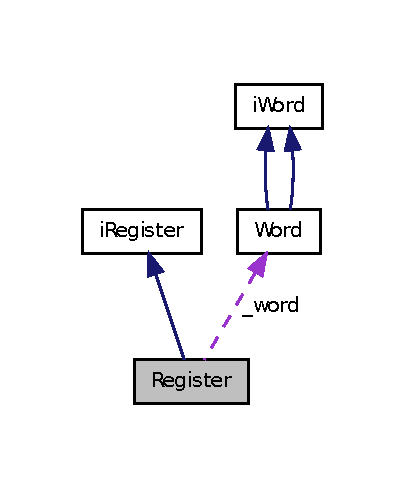
\includegraphics[width=197pt]{classRegister__coll__graph}
\end{center}
\end{figure}
\subsection*{Public Member Functions}
\begin{DoxyCompactItemize}
\item 
\hypertarget{classRegister_a73d8564754d7ddb7e8349001010e688b}{
void {\bfseries Add} (const \hyperlink{classiWord}{iWord} \&w)}
\label{classRegister_a73d8564754d7ddb7e8349001010e688b}

\item 
\hypertarget{classRegister_a9d9c6801db55e8706eb242b1e0e0fa3f}{
\hyperlink{classRegister}{Register} {\bfseries Add} (const \hyperlink{classiRegister}{iRegister} \&r) const }
\label{classRegister_a9d9c6801db55e8706eb242b1e0e0fa3f}

\item 
\hypertarget{classRegister_a312263efb06ef459409879f5119b3b81}{
void {\bfseries And} (const \hyperlink{classiWord}{iWord} \&w)}
\label{classRegister_a312263efb06ef459409879f5119b3b81}

\item 
\hypertarget{classRegister_af3502239502c214b8c9362a6fd9f8ff8}{
\hyperlink{classRegister}{Register} {\bfseries And} (const \hyperlink{classiRegister}{iRegister} \&r) const }
\label{classRegister_af3502239502c214b8c9362a6fd9f8ff8}

\item 
\hypertarget{classRegister_a379734c28ab8258ce528a96de24cfa1a}{
\hyperlink{classWord}{Word} {\bfseries GetValue} () const }
\label{classRegister_a379734c28ab8258ce528a96de24cfa1a}

\item 
\hypertarget{classRegister_abbf5f6793328db8b28845cac84c0e82d}{
void {\bfseries Not} ()}
\label{classRegister_abbf5f6793328db8b28845cac84c0e82d}

\item 
\hypertarget{classRegister_a387bb50d01b47071c366708ea10ebdf0}{
\hyperlink{classRegister}{Register} {\bfseries Not} () const }
\label{classRegister_a387bb50d01b47071c366708ea10ebdf0}

\item 
\hypertarget{classRegister_a55de0c3b5f8fe14df7c24bce777204e0}{
\hyperlink{classRegister}{Register} {\bfseries operator+} (const \hyperlink{classiRegister}{iRegister} \&r) const }
\label{classRegister_a55de0c3b5f8fe14df7c24bce777204e0}

\item 
\hypertarget{classRegister_ac4e78cff131bc5c69695a9db5ca35255}{
\hyperlink{classRegister}{Register} \& {\bfseries operator++} ()}
\label{classRegister_ac4e78cff131bc5c69695a9db5ca35255}

\item 
\hypertarget{classRegister_ae3414befdccf70a18df0f67dc19d86b7}{
\hyperlink{classRegister}{Register} \& {\bfseries operator++} (int)}
\label{classRegister_ae3414befdccf70a18df0f67dc19d86b7}

\item 
\hypertarget{classRegister_a43c957e4b6a3103f0634258891c82b46}{
\hyperlink{classRegister}{Register} {\bfseries operator-\/} (const \hyperlink{classiRegister}{iRegister} \&r) const }
\label{classRegister_a43c957e4b6a3103f0634258891c82b46}

\item 
\hypertarget{classRegister_afc5f775405700146638e392d81ad7d0b}{
\hyperlink{classRegister}{Register} \& {\bfseries operator=} (const \hyperlink{classiWord}{iWord} \&w)}
\label{classRegister_afc5f775405700146638e392d81ad7d0b}

\item 
\hypertarget{classRegister_a00f7aaf798102e5c7a6fb311551b492f}{
\hyperlink{classRegister}{Register} \& {\bfseries operator=} (const \hyperlink{classRegister}{Register} r)}
\label{classRegister_a00f7aaf798102e5c7a6fb311551b492f}

\item 
\hypertarget{classRegister_ab2f8407fab157d8deea936fa74424115}{
void {\bfseries Or} (const \hyperlink{classiWord}{iWord} \&w)}
\label{classRegister_ab2f8407fab157d8deea936fa74424115}

\item 
\hypertarget{classRegister_a9400801cc625144c4606cd7f5cbbaa21}{
\hyperlink{classRegister}{Register} {\bfseries Or} (const \hyperlink{classiRegister}{iRegister} \&r) const }
\label{classRegister_a9400801cc625144c4606cd7f5cbbaa21}

\item 
\hypertarget{classRegister_a6aea43b4c4ad669073f20fbcd274b49c}{
{\bfseries Register} (const \hyperlink{classWord}{Word} w)}
\label{classRegister_a6aea43b4c4ad669073f20fbcd274b49c}

\item 
\hypertarget{classRegister_affcc16cc88cdc896803b1ab6af5d38e0}{
void {\bfseries Store} (const \hyperlink{classiWord}{iWord} \&w)}
\label{classRegister_affcc16cc88cdc896803b1ab6af5d38e0}

\item 
\hypertarget{classRegister_a2ac7bd6f2e0eb38800c0a8c8d045e18e}{
void {\bfseries Store} (const \hyperlink{classiRegister}{iRegister} \&r)}
\label{classRegister_a2ac7bd6f2e0eb38800c0a8c8d045e18e}

\item 
\hypertarget{classRegister_a05132a4a62f5c6883fdf78731970ab6a}{
\hyperlink{classRegister}{Register} {\bfseries Subtract} (const \hyperlink{classiRegister}{iRegister} \&r) const }
\label{classRegister_a05132a4a62f5c6883fdf78731970ab6a}

\item 
\hypertarget{classRegister_a726a720b6bcca282945f1c0a65ca0dd4}{
void {\bfseries Subtract} (const \hyperlink{classiWord}{iWord} \&w)}
\label{classRegister_a726a720b6bcca282945f1c0a65ca0dd4}

\end{DoxyCompactItemize}
\subsection*{Private Attributes}
\begin{DoxyCompactItemize}
\item 
\hypertarget{classRegister_ad716faf568aba3da6e4acca6674f9ec9}{
\hyperlink{classWord}{Word} \hyperlink{classRegister_ad716faf568aba3da6e4acca6674f9ec9}{\_\-word}}
\label{classRegister_ad716faf568aba3da6e4acca6674f9ec9}

\begin{DoxyCompactList}\small\item\em The word of data held in the register. \item\end{DoxyCompactList}\end{DoxyCompactItemize}


\subsection{Detailed Description}
Implements \hyperlink{classiRegister}{iRegister}. 
\hypertarget{classWord}{
\section{Word Class Reference}
\label{classWord}\index{Word@{Word}}
}


Inheritance diagram for Word:\nopagebreak
\begin{figure}[H]
\begin{center}
\leavevmode
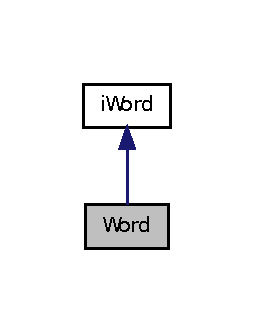
\includegraphics[width=122pt]{classWord__inherit__graph}
\end{center}
\end{figure}


Collaboration diagram for Word:\nopagebreak
\begin{figure}[H]
\begin{center}
\leavevmode
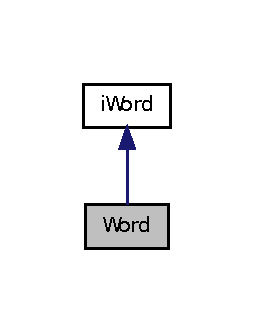
\includegraphics[width=122pt]{classWord__coll__graph}
\end{center}
\end{figure}
\subsection*{Public Member Functions}
\begin{DoxyCompactItemize}
\item 
int \hyperlink{classWord_a19303d963626549830a8da33d863bd6d}{toInt} () const 
\begin{DoxyCompactList}\small\item\em \char`\"{}To non-\/negative Integer\char`\"{} \item\end{DoxyCompactList}\item 
int \hyperlink{classWord_a3d771d68afd4a70d279af8bd9cd6bef9}{toInt2Complement} () const 
\begin{DoxyCompactList}\small\item\em \char`\"{}To Integer as 2's Complement\char`\"{} \item\end{DoxyCompactList}\item 
std::string \hyperlink{classWord_ac2ca49ef4da2fb57172fe057849e53fa}{toStr} () const 
\begin{DoxyCompactList}\small\item\em \char`\"{}To String\char`\"{} \item\end{DoxyCompactList}\item 
std::string \hyperlink{classWord_ab797467868642bb096bc4c9b1ed0a2f0}{toHex} () const 
\begin{DoxyCompactList}\small\item\em \char`\"{}To Hexadecimal\char`\"{} \item\end{DoxyCompactList}\item 
bool \hyperlink{classWord_ad6499f93b487d6d550a3fd4adcee9c8d}{fromInt} (int)
\begin{DoxyCompactList}\small\item\em \char`\"{}From Integer\char`\"{} \item\end{DoxyCompactList}\item 
bool \hyperlink{classWord_a614b52f3312d82ac5681403651040714}{fromStr} (const std::string \&)
\begin{DoxyCompactList}\small\item\em \char`\"{}From String\char`\"{} \item\end{DoxyCompactList}\item 
bool \hyperlink{classWord_a4e26eb82e8f7426dd46be2bbec9e41c5}{fromHex} (const std::string \&)
\begin{DoxyCompactList}\small\item\em \char`\"{}From Hexadecimal\char`\"{} \item\end{DoxyCompactList}\item 
\hyperlink{classWord}{Word} \hyperlink{classWord_a5cb9115a6cee6666e88390e56eb32071}{Add} (const \hyperlink{classiWord}{iWord} \&) const 
\begin{DoxyCompactList}\small\item\em Adds two words. \item\end{DoxyCompactList}\item 
\hyperlink{classWord}{Word} \hyperlink{classWord_a88e945efd81d13e15adb1ed9e4e95a5a}{operator+} (const \hyperlink{classiWord}{iWord} \&) const 
\begin{DoxyCompactList}\small\item\em A standard addition operator. \item\end{DoxyCompactList}\item 
\hyperlink{classWord}{Word} \hyperlink{classWord_a3ef457fb6f6ce54f5e98a83db4ae4472}{Subtract} (const \hyperlink{classiWord}{iWord} \&) const 
\begin{DoxyCompactList}\small\item\em Subtracts two words. \item\end{DoxyCompactList}\item 
\hyperlink{classWord}{Word} \hyperlink{classWord_a9ec270f103a3a755bd7b627e4b899bb4}{operator-\/} (const \hyperlink{classiWord}{iWord} \&) const 
\begin{DoxyCompactList}\small\item\em A standard subtraction operator. \item\end{DoxyCompactList}\item 
\hyperlink{classWord}{Word} \hyperlink{classWord_a4e1926ab5f4af7b63ec1bf4fadf873ad}{And} (const \hyperlink{classiWord}{iWord} \&) const 
\begin{DoxyCompactList}\small\item\em \char`\"{}And\char`\"{}s the bits of two words. \item\end{DoxyCompactList}\item 
\hypertarget{classWord_aa8645b9198fac6d0833b32503db6e18a}{
\hyperlink{classWord}{Word} {\bfseries Or} (const \hyperlink{classiWord}{iWord} \&) const }
\label{classWord_aa8645b9198fac6d0833b32503db6e18a}

\item 
\hypertarget{classWord_afdecfa9e3f2fda36496f249617a4cef5}{
\hyperlink{classWord}{Word} {\bfseries Not} () const }
\label{classWord_afdecfa9e3f2fda36496f249617a4cef5}

\item 
void \hyperlink{classWord_abb97142e332c7cc25d2a0c2bdb6c3d9b}{copy} (const \hyperlink{classiWord}{iWord} \&)
\begin{DoxyCompactList}\small\item\em Copies a word. \item\end{DoxyCompactList}\item 
\hyperlink{classWord}{Word} \& \hyperlink{classWord_a2ae41869cb0f1855fc18c6bce05f7c4d}{operator=} (const \hyperlink{classWord}{Word})
\begin{DoxyCompactList}\small\item\em A standard assignment operator. \item\end{DoxyCompactList}\item 
\hyperlink{classiWord}{iWord} \& \hyperlink{classWord_a3837f49bcb44597e6d738ccb0eeed144}{operator++} ()
\item 
\hyperlink{classiWord}{iWord} \& \hyperlink{classWord_ae921b75d263be790fd150c5962445163}{operator++} (int)
\begin{DoxyCompactList}\small\item\em A standard post-\/increment operator. \item\end{DoxyCompactList}\item 
bool \hyperlink{classWord_ab0f10ac1a0397559b859774b503538fe}{operator\mbox{[}$\,$\mbox{]}} (const int) const 
\begin{DoxyCompactList}\small\item\em An accessor to the \char`\"{}i\char`\"{}th bit of the value. \item\end{DoxyCompactList}\item 
\hypertarget{classWord_a7484e0f4d1fa712ca367539dad71dfa3}{
void {\bfseries print} () const }
\label{classWord_a7484e0f4d1fa712ca367539dad71dfa3}

\end{DoxyCompactItemize}
\subsection*{Private Member Functions}
\begin{DoxyCompactItemize}
\item 
\hypertarget{classWord_aaacae836ba9ed28f9725432ae81ab318}{
bool {\bfseries \_\-hasBit} (int) const }
\label{classWord_aaacae836ba9ed28f9725432ae81ab318}

\end{DoxyCompactItemize}
\subsection*{Private Attributes}
\begin{DoxyCompactItemize}
\item 
\hypertarget{classWord_a8b0aa1f2042266f307c51b3bdafa9128}{
unsigned short {\bfseries \_\-value}}
\label{classWord_a8b0aa1f2042266f307c51b3bdafa9128}

\end{DoxyCompactItemize}


\subsection{Member Function Documentation}
\hypertarget{classWord_a19303d963626549830a8da33d863bd6d}{
\index{Word@{Word}!toInt@{toInt}}
\index{toInt@{toInt}!Word@{Word}}
\subsubsection[{toInt}]{\setlength{\rightskip}{0pt plus 5cm}int Word::toInt (
\begin{DoxyParamCaption}
{}
\end{DoxyParamCaption}
) const\hspace{0.3cm}{\ttfamily  \mbox{[}virtual\mbox{]}}}}
\label{classWord_a19303d963626549830a8da33d863bd6d}


\char`\"{}To non-\/negative Integer\char`\"{} 

\begin{DoxyPostcond}{Postcondition}
The value of the word is not changed. 
\end{DoxyPostcond}
\begin{DoxyReturn}{Returns}
The bits of the word interpreted as a positive integer value. 
\end{DoxyReturn}


Implements \hyperlink{classiWord_a3349d0a243d3432bb35b76af8420b1d9}{iWord}.

\hypertarget{classWord_a3d771d68afd4a70d279af8bd9cd6bef9}{
\index{Word@{Word}!toInt2Complement@{toInt2Complement}}
\index{toInt2Complement@{toInt2Complement}!Word@{Word}}
\subsubsection[{toInt2Complement}]{\setlength{\rightskip}{0pt plus 5cm}int Word::toInt2Complement (
\begin{DoxyParamCaption}
{}
\end{DoxyParamCaption}
) const\hspace{0.3cm}{\ttfamily  \mbox{[}virtual\mbox{]}}}}
\label{classWord_a3d771d68afd4a70d279af8bd9cd6bef9}


\char`\"{}To Integer as 2's Complement\char`\"{} 

\begin{DoxyPostcond}{Postcondition}
The value of the word is not changed. 
\end{DoxyPostcond}
\begin{DoxyReturn}{Returns}
The bits of the word interpreted as a signed (2's complement) integer value. 
\end{DoxyReturn}


Implements \hyperlink{classiWord_a1377d01257b792c748b013be60b089e6}{iWord}.

\hypertarget{classWord_ac2ca49ef4da2fb57172fe057849e53fa}{
\index{Word@{Word}!toStr@{toStr}}
\index{toStr@{toStr}!Word@{Word}}
\subsubsection[{toStr}]{\setlength{\rightskip}{0pt plus 5cm}string Word::toStr (
\begin{DoxyParamCaption}
{}
\end{DoxyParamCaption}
) const\hspace{0.3cm}{\ttfamily  \mbox{[}virtual\mbox{]}}}}
\label{classWord_ac2ca49ef4da2fb57172fe057849e53fa}


\char`\"{}To String\char`\"{} 

\begin{DoxyPostcond}{Postcondition}
The value of the word is not changed. 
\end{DoxyPostcond}
\begin{DoxyReturn}{Returns}
\char`\"{}\mbox{[}\char`\"{} + $<$16 characters: either 1's or 0's$>$ + \char`\"{}\mbox{]}\char`\"{}
\end{DoxyReturn}
\begin{DoxyParagraph}{Examples:}
If the object holds a (2's comp.) value 4: \mbox{[}0000000000000100\mbox{]}\par
 If the object holds a (2's comp.) value -\/1: \mbox{[}1111111111111111\mbox{]} 
\end{DoxyParagraph}


Implements \hyperlink{classiWord_a0114861c4b660286834ad637f11dc4f4}{iWord}.

\hypertarget{classWord_ab797467868642bb096bc4c9b1ed0a2f0}{
\index{Word@{Word}!toHex@{toHex}}
\index{toHex@{toHex}!Word@{Word}}
\subsubsection[{toHex}]{\setlength{\rightskip}{0pt plus 5cm}string Word::toHex (
\begin{DoxyParamCaption}
{}
\end{DoxyParamCaption}
) const\hspace{0.3cm}{\ttfamily  \mbox{[}virtual\mbox{]}}}}
\label{classWord_ab797467868642bb096bc4c9b1ed0a2f0}


\char`\"{}To Hexadecimal\char`\"{} 

\begin{DoxyPostcond}{Postcondition}
The value of the word is not changed. 
\end{DoxyPostcond}
\begin{DoxyReturn}{Returns}
\char`\"{}0x\char`\"{} + $<$4 characters in the range \mbox{[}0-\/9\mbox{]},\mbox{[}A-\/F\mbox{]}$>$
\end{DoxyReturn}
\begin{DoxyParagraph}{Examples:}
If the object holds (2's comp.) value 8: 0x0008\par
 If the object holds (2's comp.) value -\/2: 0xFFFE 
\end{DoxyParagraph}


Implements \hyperlink{classiWord_a7fc28d0251f8acb4dc3f388fc25c57d1}{iWord}.

\hypertarget{classWord_ad6499f93b487d6d550a3fd4adcee9c8d}{
\index{Word@{Word}!fromInt@{fromInt}}
\index{fromInt@{fromInt}!Word@{Word}}
\subsubsection[{fromInt}]{\setlength{\rightskip}{0pt plus 5cm}bool Word::fromInt (
\begin{DoxyParamCaption}
\item[{int}]{}
\end{DoxyParamCaption}
)\hspace{0.3cm}{\ttfamily  \mbox{[}virtual\mbox{]}}}}
\label{classWord_ad6499f93b487d6d550a3fd4adcee9c8d}


\char`\"{}From Integer\char`\"{} 


\begin{DoxyParams}[1]{Parameters}
\mbox{\tt in}  & {\em value} & The value to be stored into the word. \\
\hline
\end{DoxyParams}
\begin{DoxyPostcond}{Postcondition}
\char`\"{}value\char`\"{} is not changed. 
\end{DoxyPostcond}
\begin{DoxyReturn}{Returns}
True if and only if \char`\"{}value\char`\"{} can be represented in 16 bits
\end{DoxyReturn}
When this function returns \char`\"{}False\char`\"{}, the value of the word is unchanged.\par
 Otherwise, the word now holds the value \char`\"{}value\char`\"{}. 

Implements \hyperlink{classiWord_a6421bf139c6eb4044446997606cb65e7}{iWord}.

\hypertarget{classWord_a614b52f3312d82ac5681403651040714}{
\index{Word@{Word}!fromStr@{fromStr}}
\index{fromStr@{fromStr}!Word@{Word}}
\subsubsection[{fromStr}]{\setlength{\rightskip}{0pt plus 5cm}bool Word::fromStr (
\begin{DoxyParamCaption}
\item[{const std::string \&}]{}
\end{DoxyParamCaption}
)\hspace{0.3cm}{\ttfamily  \mbox{[}virtual\mbox{]}}}}
\label{classWord_a614b52f3312d82ac5681403651040714}


\char`\"{}From String\char`\"{} 


\begin{DoxyParams}[1]{Parameters}
\mbox{\tt in}  & {\em str} & A string of characters meant to represent a \char`\"{}word\char`\"{} to be stored. \\
\hline
\end{DoxyParams}
\begin{DoxyPostcond}{Postcondition}
\char`\"{}str\char`\"{} is not changed. 
\end{DoxyPostcond}
\begin{DoxyReturn}{Returns}
True if and only if \char`\"{}str\char`\"{} is well-\/formed (as defined in \hyperlink{classWord_ac2ca49ef4da2fb57172fe057849e53fa}{toStr()}).
\end{DoxyReturn}
When this function returns \char`\"{}False\char`\"{}, the value of the word is unchanged.\par
 Otherwise, the word now holds the value \char`\"{}str\char`\"{}. 

Implements \hyperlink{classiWord_ad8df9e06ccb87d1e65766120713ef545}{iWord}.

\hypertarget{classWord_a4e26eb82e8f7426dd46be2bbec9e41c5}{
\index{Word@{Word}!fromHex@{fromHex}}
\index{fromHex@{fromHex}!Word@{Word}}
\subsubsection[{fromHex}]{\setlength{\rightskip}{0pt plus 5cm}bool Word::fromHex (
\begin{DoxyParamCaption}
\item[{const std::string \&}]{}
\end{DoxyParamCaption}
)\hspace{0.3cm}{\ttfamily  \mbox{[}virtual\mbox{]}}}}
\label{classWord_a4e26eb82e8f7426dd46be2bbec9e41c5}


\char`\"{}From Hexadecimal\char`\"{} 


\begin{DoxyParams}[1]{Parameters}
\mbox{\tt in}  & {\em str} & A string of characters meant to represent a \char`\"{}word\char`\"{} to be stored. \\
\hline
\end{DoxyParams}
\begin{DoxyPostcond}{Postcondition}
\char`\"{}str\char`\"{} is not changed. 
\end{DoxyPostcond}
\begin{DoxyReturn}{Returns}
True if and only if \char`\"{}str\char`\"{} is well-\/formed (as defined in \hyperlink{classWord_ab797467868642bb096bc4c9b1ed0a2f0}{toHex()}).
\end{DoxyReturn}
When this function returns \char`\"{}False\char`\"{}, the value of the word is unchanged.\par
 Otherwise, the word now holds the value \char`\"{}str\char`\"{}. 

Implements \hyperlink{classiWord_a0c08832b3e9b41073fc6666407ef8c53}{iWord}.

\hypertarget{classWord_a5cb9115a6cee6666e88390e56eb32071}{
\index{Word@{Word}!Add@{Add}}
\index{Add@{Add}!Word@{Word}}
\subsubsection[{Add}]{\setlength{\rightskip}{0pt plus 5cm}{\bf Word} Word::Add (
\begin{DoxyParamCaption}
\item[{const {\bf iWord} \&}]{}
\end{DoxyParamCaption}
) const\hspace{0.3cm}{\ttfamily  \mbox{[}virtual\mbox{]}}}}
\label{classWord_a5cb9115a6cee6666e88390e56eb32071}


Adds two words. 


\begin{DoxyParams}[1]{Parameters}
\mbox{\tt in}  & {\em w} & A word value to be added. \\
\hline
\end{DoxyParams}
\begin{DoxyPostcond}{Postcondition}
Both \char`\"{}w\char`\"{} and the calling object do not change. 
\end{DoxyPostcond}
\begin{DoxyReturn}{Returns}
A new \char`\"{}Word\char`\"{} object containing result of adding \char`\"{}w\char`\"{} and the calling object.
\end{DoxyReturn}
\begin{DoxyNote}{Note}
The addition is carried out with no regard to logical overflow. 
\end{DoxyNote}


Implements \hyperlink{classiWord_a999c52ac2e7abf756eeb16fe5b31aad7}{iWord}.

\hypertarget{classWord_a88e945efd81d13e15adb1ed9e4e95a5a}{
\index{Word@{Word}!operator+@{operator+}}
\index{operator+@{operator+}!Word@{Word}}
\subsubsection[{operator+}]{\setlength{\rightskip}{0pt plus 5cm}{\bf Word} Word::operator+ (
\begin{DoxyParamCaption}
\item[{const {\bf iWord} \&}]{}
\end{DoxyParamCaption}
) const\hspace{0.3cm}{\ttfamily  \mbox{[}virtual\mbox{]}}}}
\label{classWord_a88e945efd81d13e15adb1ed9e4e95a5a}


A standard addition operator. 

\begin{DoxyNote}{Note}
\char`\"{}result = p + w\char`\"{} is equivalent to \char`\"{}result = p.Add(w)\char`\"{}. 
\end{DoxyNote}


Implements \hyperlink{classiWord_a8dfb66b7cd91fe0a4169f071c1f9bc53}{iWord}.

\hypertarget{classWord_a3ef457fb6f6ce54f5e98a83db4ae4472}{
\index{Word@{Word}!Subtract@{Subtract}}
\index{Subtract@{Subtract}!Word@{Word}}
\subsubsection[{Subtract}]{\setlength{\rightskip}{0pt plus 5cm}{\bf Word} Word::Subtract (
\begin{DoxyParamCaption}
\item[{const {\bf iWord} \&}]{}
\end{DoxyParamCaption}
) const\hspace{0.3cm}{\ttfamily  \mbox{[}virtual\mbox{]}}}}
\label{classWord_a3ef457fb6f6ce54f5e98a83db4ae4472}


Subtracts two words. 


\begin{DoxyParams}[1]{Parameters}
\mbox{\tt in}  & {\em w} & A word value to be subtracted. \\
\hline
\end{DoxyParams}
\begin{DoxyPostcond}{Postcondition}
Both \char`\"{}w\char`\"{} and the calling object do not change. 
\end{DoxyPostcond}
\begin{DoxyReturn}{Returns}
A new \char`\"{}Word\char`\"{} object containing the result of subtracting \char`\"{}w\char`\"{} from the calling object.
\end{DoxyReturn}
\begin{DoxyNote}{Note}
The subtraction is carried out with no regard for logical overflow. 
\end{DoxyNote}


Implements \hyperlink{classiWord_af69a5e10e094e3fc30fae0b651d95ea6}{iWord}.

\hypertarget{classWord_a9ec270f103a3a755bd7b627e4b899bb4}{
\index{Word@{Word}!operator-\/@{operator-\/}}
\index{operator-\/@{operator-\/}!Word@{Word}}
\subsubsection[{operator-\/}]{\setlength{\rightskip}{0pt plus 5cm}{\bf Word} Word::operator-\/ (
\begin{DoxyParamCaption}
\item[{const {\bf iWord} \&}]{}
\end{DoxyParamCaption}
) const\hspace{0.3cm}{\ttfamily  \mbox{[}virtual\mbox{]}}}}
\label{classWord_a9ec270f103a3a755bd7b627e4b899bb4}


A standard subtraction operator. 

\begin{DoxyNote}{Note}
\char`\"{}result = p -\/ w\char`\"{} is equivalent to \char`\"{}result = p.Subtract(w)\char`\"{}. 
\end{DoxyNote}


Implements \hyperlink{classiWord_a432fb05081debadb601d86cca05152c8}{iWord}.

\hypertarget{classWord_a4e1926ab5f4af7b63ec1bf4fadf873ad}{
\index{Word@{Word}!And@{And}}
\index{And@{And}!Word@{Word}}
\subsubsection[{And}]{\setlength{\rightskip}{0pt plus 5cm}{\bf Word} Word::And (
\begin{DoxyParamCaption}
\item[{const {\bf iWord} \&}]{}
\end{DoxyParamCaption}
) const\hspace{0.3cm}{\ttfamily  \mbox{[}virtual\mbox{]}}}}
\label{classWord_a4e1926ab5f4af7b63ec1bf4fadf873ad}


\char`\"{}And\char`\"{}s the bits of two words. 


\begin{DoxyParams}[1]{Parameters}
\mbox{\tt in}  & {\em w} & A word value to be \char`\"{}and\char`\"{}ed. \\
\hline
\end{DoxyParams}
\begin{DoxyPostcond}{Postcondition}
Both \char`\"{}w\char`\"{} and the calling object do not change. 
\end{DoxyPostcond}
\begin{DoxyReturn}{Returns}
A new \char`\"{}Word\char`\"{} object containing the result of performing a bit-\/wise and on \char`\"{}w\char`\"{} and the calling object. 
\end{DoxyReturn}


Implements \hyperlink{classiWord_ae9f6bbc855712a208835d12cb3e40577}{iWord}.

\hypertarget{classWord_abb97142e332c7cc25d2a0c2bdb6c3d9b}{
\index{Word@{Word}!copy@{copy}}
\index{copy@{copy}!Word@{Word}}
\subsubsection[{copy}]{\setlength{\rightskip}{0pt plus 5cm}void Word::copy (
\begin{DoxyParamCaption}
\item[{const {\bf iWord} \&}]{}
\end{DoxyParamCaption}
)\hspace{0.3cm}{\ttfamily  \mbox{[}virtual\mbox{]}}}}
\label{classWord_abb97142e332c7cc25d2a0c2bdb6c3d9b}


Copies a word. 


\begin{DoxyParams}[1]{Parameters}
\mbox{\tt out}  & {\em The} & value to be copied. \\
\hline
\end{DoxyParams}
\begin{DoxyPostcond}{Postcondition}
The caller equals that parameter.
\end{DoxyPostcond}
Equivalent to the assignment \char`\"{}caller = parameter\char`\"{}. 

Implements \hyperlink{classiWord_ab9f5df8ced4937c18f16784a98ecf95f}{iWord}.

\hypertarget{classWord_a2ae41869cb0f1855fc18c6bce05f7c4d}{
\index{Word@{Word}!operator=@{operator=}}
\index{operator=@{operator=}!Word@{Word}}
\subsubsection[{operator=}]{\setlength{\rightskip}{0pt plus 5cm}{\bf Word} \& Word::operator= (
\begin{DoxyParamCaption}
\item[{const }]{ Word}
\end{DoxyParamCaption}
)\hspace{0.3cm}{\ttfamily  \mbox{[}virtual\mbox{]}}}}
\label{classWord_a2ae41869cb0f1855fc18c6bce05f7c4d}


A standard assignment operator. 


\begin{DoxyParams}[1]{Parameters}
\mbox{\tt in}  & {\em The} & value to be copied. \\
\hline
\end{DoxyParams}
\begin{DoxyReturn}{Returns}
A copy of the parameter.
\end{DoxyReturn}
The return value and parameter here must be declared as \char`\"{}Word\char`\"{}s as C++ does not work well with polymorphic assignment operators. 

Implements \hyperlink{classiWord_a45c9c82054bd2150b77d5f157734cb72}{iWord}.

\hypertarget{classWord_a3837f49bcb44597e6d738ccb0eeed144}{
\index{Word@{Word}!operator++@{operator++}}
\index{operator++@{operator++}!Word@{Word}}
\subsubsection[{operator++}]{\setlength{\rightskip}{0pt plus 5cm}{\bf iWord} \& Word::operator++ (
\begin{DoxyParamCaption}
{}
\end{DoxyParamCaption}
)\hspace{0.3cm}{\ttfamily  \mbox{[}virtual\mbox{]}}}}
\label{classWord_a3837f49bcb44597e6d738ccb0eeed144}
A standard pre-\/increment operator. \begin{DoxyReturn}{Returns}
A reference to itself.
\end{DoxyReturn}
The object increments its value BEFORE the execution of the current line. 

Implements \hyperlink{classiWord_af20040c25b79d2aeae41f1714fbb2cbc}{iWord}.

\hypertarget{classWord_ae921b75d263be790fd150c5962445163}{
\index{Word@{Word}!operator++@{operator++}}
\index{operator++@{operator++}!Word@{Word}}
\subsubsection[{operator++}]{\setlength{\rightskip}{0pt plus 5cm}{\bf iWord} \& Word::operator++ (
\begin{DoxyParamCaption}
\item[{int}]{}
\end{DoxyParamCaption}
)\hspace{0.3cm}{\ttfamily  \mbox{[}virtual\mbox{]}}}}
\label{classWord_ae921b75d263be790fd150c5962445163}


A standard post-\/increment operator. 

\begin{DoxyReturn}{Returns}
A reference to itself.
\end{DoxyReturn}
The object increments its value AFTER the execution of the current line. 

Implements \hyperlink{classiWord_a6777f6f41915179c4255d3647a9eb4b5}{iWord}.

\hypertarget{classWord_ab0f10ac1a0397559b859774b503538fe}{
\index{Word@{Word}!operator\mbox{[}\mbox{]}@{operator[]}}
\index{operator\mbox{[}\mbox{]}@{operator[]}!Word@{Word}}
\subsubsection[{operator[]}]{\setlength{\rightskip}{0pt plus 5cm}bool Word::operator\mbox{[}$\,$\mbox{]} (
\begin{DoxyParamCaption}
\item[{const }]{}
\end{DoxyParamCaption}
) const\hspace{0.3cm}{\ttfamily  \mbox{[}virtual\mbox{]}}}}
\label{classWord_ab0f10ac1a0397559b859774b503538fe}


An accessor to the \char`\"{}i\char`\"{}th bit of the value. 


\begin{DoxyParams}[1]{Parameters}
\mbox{\tt in}  & {\em The} & index of the bit in question. \\
\hline
\end{DoxyParams}
\begin{DoxyPrecond}{Precondition}
The index must be less than the size of a word, ie. 16. 
\end{DoxyPrecond}
\begin{DoxyReturn}{Returns}
True $<$=$>$ 1, False $<$=$>$ 0.
\end{DoxyReturn}
The number of the bits starts at zero and rises into the more significant bits. Examples: If the object \char`\"{}num\char`\"{} holds a value of 4 (0...100 in binary), num\mbox{[}0\mbox{]} = 0, num\mbox{[}1\mbox{]} = 0, num\mbox{[}2\mbox{]} = 1. If it holds a value of 1 (0...001 in binary) num\mbox{[}0\mbox{]} = 1, num\mbox{[}1\mbox{]} = 0, num\mbox{[}2\mbox{]} = 0, etc. If it holds a negative value (Starting with a 1 in 2's complement), num\mbox{[}15\mbox{]} = 1. 

Implements \hyperlink{classiWord_a2bd140904379329b74c3e1af83eb3a85}{iWord}.



The documentation for this class was generated from the following files:\begin{DoxyCompactItemize}
\item 
Word.h\item 
Word.cpp\end{DoxyCompactItemize}

\printindex
\end{document}
